\documentclass[a4paper,11pt]{ltjsarticle}

\usepackage[haranoaji]{luatexja-preset}
\usepackage{amsmath,amssymb,mathtools}
\usepackage{array}
\usepackage{booktabs}
\usepackage{geometry}
\usepackage{graphicx}
\usepackage{hyperref}
\usepackage{longtable}
\usepackage{tabularx}
\usepackage{tikz}
\usepackage{xcolor}
\usetikzlibrary{arrows.meta,calc,positioning}

\geometry{margin=25mm}
\hypersetup{
  colorlinks=true,
  linkcolor=blue!55!black,
  urlcolor=blue!55!black,
  citecolor=blue!55!black
}

\renewcommand{\arraystretch}{1.2}

\newcolumntype{Y}{>{\raggedright\arraybackslash}X}
\newcommand{\F}{\mathbb{F}}
\newcommand{\Setup}{\mathsf{Setup}}
\newcommand{\Com}{\mathsf{Com}}
\newcommand{\Commit}{\mathsf{Commit}}
\newcommand{\Open}{\mathsf{Open}}
\newcommand{\Verify}{\mathsf{Verify}}
\newcommand{\poly}{\mathsf{poly}}
\newcommand{\wit}{\mathsf{witness}}
\newcommand{\stmt}{\mathsf{statement}}
\newcommand{\SRS}{\mathsf{SRS}}
\newcommand{\Z}{\mathbb{Z}}
\newcommand{\G}{\mathbb{G}}
\newcommand{\GT}{\mathbb{G}_T}
\newcommand{\E}{\mathcal{E}}
\newcommand{\Hash}{\mathsf{Hash}}
\newcommand{\Ext}{\mathsf{Ext}}
\newcommand{\Sim}{\mathsf{Sim}}
\newcommand{\negl}{\mathsf{negl}}

\definecolor{NoteBlue}{HTML}{EEF5FF}
\definecolor{NoteGreen}{HTML}{EEF9F1}
\definecolor{NoteYellow}{HTML}{FFF8E6}
\definecolor{NoteRed}{HTML}{FFF0F0}
\definecolor{NoteGray}{HTML}{F6F7F9}

\newenvironment{learningbox}{%
  \paragraph*{この章で答える問い}\begin{quote}
}{%
  \end{quote}
}

\newenvironment{keybox}{%
  \paragraph*{まず覚えること}\begin{quote}
}{%
  \end{quote}
}

\newenvironment{examplebox}[1]{%
  \paragraph*{#1}\begin{quote}
}{%
  \end{quote}
}

\newenvironment{warnbox}{%
  \paragraph*{注意}\begin{quote}
}{%
  \end{quote}
}

\newenvironment{checkpointbox}{%
  \paragraph*{確認問題}\begin{quote}
}{%
  \end{quote}
}

\newenvironment{advancedbox}{%
  \paragraph*{発展内容}\begin{quote}
}{%
  \end{quote}
}

\newenvironment{diagramfigure}[1]{%
  \begin{center}
  \begin{minipage}{0.98\linewidth}
  \centering
  {\small\textbf{#1}\par}\medskip
}{%
  \end{minipage}
  \end{center}
}

\tikzset{
  zknode/.style={draw=blue!55!black, fill=NoteBlue, rounded corners=2pt, align=center, inner sep=4pt, font=\normalsize},
  zkgreen/.style={draw=green!40!black, fill=NoteGreen, rounded corners=2pt, align=center, inner sep=4pt, font=\normalsize},
  zkyellow/.style={draw=yellow!45!black, fill=NoteYellow, rounded corners=2pt, align=center, inner sep=4pt, font=\normalsize},
  zkred/.style={draw=red!45!black, fill=NoteRed, rounded corners=2pt, align=center, inner sep=4pt, font=\normalsize},
  zkgray/.style={draw=gray!65!black, fill=NoteGray, rounded corners=2pt, align=center, inner sep=4pt, font=\normalsize},
  zkhash/.style={draw=blue!50!black, fill=NoteBlue, circle, minimum size=8mm, align=center, font=\normalsize},
  zkarrow/.style={-{Latex[length=2mm]}, thick, draw=blue!55!black},
  zksoftarrow/.style={-{Latex[length=2mm]}, thick, draw=gray!65!black},
  zkdotarrow/.style={-{Latex[length=2mm]}, dashed, thick, draw=gray!65!black}
}

\newcommand{\DiagramProverVerifier}{%
\begin{diagramfigure}{ProverとVerifierの見える関係}
\begin{tikzpicture}[node distance=8mm and 16mm]
  \node[zkgray, text width=30mm, minimum height=12mm] (prover) {Prover\\証明者};
  \node[zkgray, text width=30mm, minimum height=12mm, right=58mm of prover] (verifier) {Verifier\\検証者};
  \node[zkred, text width=32mm, below=of prover] (witness) {鍵付きの箱\\witness \(w\)};
  \node[zkgreen, text width=78mm, above=9mm of $(prover)!0.5!(verifier)$] (statement) {公開されたstatement \(x\)};
  \node[zknode, text width=25mm, below=of $(prover)!0.5!(verifier)$] (proof) {proof\\ \(\pi\)};
  \node[zkyellow, text width=36mm, below=of verifier] (check) {\(\Verify(x,\pi)=1\)};
  \draw[zksoftarrow] (statement.south west) -- (prover.north);
  \draw[zksoftarrow] (statement.south east) -- (verifier.north);
  \draw[zkarrow] (witness) -- (proof);
  \draw[zkarrow] (proof) -- (check);
  \draw[zkdotarrow] (witness.east) to[bend right=16] node[below,font=\scriptsize] {ここは渡さない} (verifier.south);
\end{tikzpicture}
\end{diagramfigure}
}

\newcommand{\DiagramWaldoZk}{%
\begin{diagramfigure}{場所を見せずに「知っている」と納得させる}
\begin{tikzpicture}[x=6mm,y=6mm]
  \node[font=\small] at (2.5,4.7) {全体の絵};
  \foreach \x in {0,...,5} {
    \foreach \y in {0,...,3} {
      \draw[fill=NoteGray, draw=gray!55] (\x,\y) rectangle ++(1,1);
    }
  }
  \fill[red!65] (3.5,2.5) circle (0.22);
  \node[font=\scriptsize] at (3.5,2.5) {?};
  \node[font=\small] at (12,4.7) {proofとして見せるもの};
  \draw[fill=black!80, draw=black] (9,0) rectangle ++(6,4);
  \draw[fill=white, draw=yellow!60!black, line width=1pt] (12,2) rectangle ++(1,1);
  \fill[red!65] (12.5,2.5) circle (0.22);
  \node[font=\scriptsize] at (12.5,2.5) {?};
  \draw[zkarrow] (6.4,2) -- node[above,font=\scriptsize] {位置は隠す} (8.5,2);
  \node[font=\scriptsize, align=center] at (12, -0.7) {周囲を隠した窓だけを見せる\\検証者は対象の存在を確認できる};
\end{tikzpicture}
\end{diagramfigure}
}

\newcommand{\DiagramSigmaProtocol}{%
\begin{diagramfigure}{離散対数の知識証明: 三つのメッセージ}
\begin{tikzpicture}[node distance=7mm and 20mm]
  \node[zkgray, text width=24mm] (p) {Prover\\秘密 \(x\)};
  \node[zkgray, text width=24mm, right=72mm of p] (v) {Verifier\\公開 \(g,y\)};
  \coordinate (p1) at ($(p.south)+(0,-8mm)$);
  \coordinate (v1) at ($(v.south)+(0,-8mm)$);
  \coordinate (p2) at ($(p1)+(0,-9mm)$);
  \coordinate (v2) at ($(v1)+(0,-9mm)$);
  \coordinate (p3) at ($(p2)+(0,-9mm)$);
  \coordinate (v3) at ($(v2)+(0,-9mm)$);
  \draw[zkarrow] (p1) -- node[above] {\(a=g^r\)} (v1);
  \draw[zkarrow] (v2) -- node[above] {challenge \(b\)} (p2);
  \draw[zkarrow] (p3) -- node[above] {\(c=r+bx\)} (v3);
  \node[zkyellow, text width=44mm, below=15mm of v] (check) {検証\\ \(g^c=ay^b\)};
  \node[zkred, text width=52mm, below=11mm of p] (extract) {同じ \(a\) に二通り答えられるなら\\ \(x=c_1-c_0\)};
  \draw[zksoftarrow] (v3) -- (check);
\end{tikzpicture}
\end{diagramfigure}
}

\newcommand{\DiagramFiniteFieldClock}{%
\begin{diagramfigure}{F7の計算は時計のように回る}
\begin{tikzpicture}[scale=0.95]
  \foreach \i in {0,...,6} {
    \node[draw=blue!55!black, fill=NoteBlue, circle, minimum size=8mm] (n\i) at ({90-360*\i/7}:2.1) {\i};
  }
  \draw[zkarrow] (n5) to[bend left=18] node[below left] {+6} (n4);
  \draw[zkarrow] (n3) to[out=10,in=-25,looseness=1.45] node[right,xshift=2mm] {x5} (n1);
  \node[align=center] at (5.2,0.5) {5+6=11, 余り4\\3x5=15, 余り1};
\end{tikzpicture}
\end{diagramfigure}
}

\newcommand{\DiagramFftButterfly}{%
\begin{diagramfigure}{FFTの蝶形: 偶数次と奇数次を合流させる}
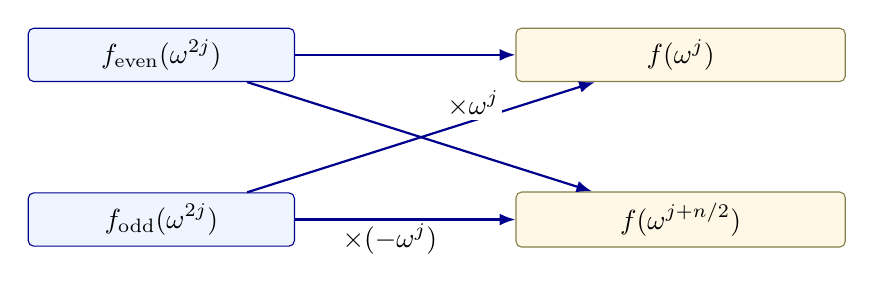
\begin{tikzpicture}[node distance=14mm and 28mm]
  \node[zknode, text width=31mm] (even) {\(\displaystyle f_{\mathrm{even}}(\omega^{2j})\)};
  \node[zknode, text width=31mm, below=of even] (odd) {\(\displaystyle f_{\mathrm{odd}}(\omega^{2j})\)};
  \node[zkyellow, text width=39mm, right=of even] (top) {\(\displaystyle f(\omega^j)\)};
  \node[zkyellow, text width=39mm, right=of odd] (bottom) {\(\displaystyle f(\omega^{j+n/2})\)};
  \draw[zkarrow] (even) -- (top);
  \draw[zkarrow] (odd) -- node[pos=0.65,above,fill=white,inner sep=1pt,font=\normalsize] {\(\displaystyle \times\omega^j\)} (top);
  \draw[zkarrow] (even) -- (bottom);
  \draw[zkarrow] (odd) -- node[pos=0.43,below,fill=white,inner sep=1pt,font=\normalsize] {\(\displaystyle \times(-\omega^j)\)} (bottom);
\end{tikzpicture}
\end{diagramfigure}
}

\newcommand{\DiagramEllipticAddition}{%
\begin{diagramfigure}{楕円曲線の点加算: 直線で交わり、上下を反転する}
\begin{tikzpicture}[x=13mm,y=13mm]
  \draw[->, gray!60] (-3,0) -- (3.2,0);
  \draw[->, gray!60] (0,-2.1) -- (0,2.1);
  \draw[blue!65!black, thick, domain=-2.1:2.1, samples=100, smooth] plot (\x,{0.28*(\x*\x*\x-\x)});
  \coordinate (P) at (-1.55,-0.62);
  \coordinate (Q) at (0.85,-0.03);
  \coordinate (minusR) at (1.65,0.75);
  \coordinate (R) at (1.65,-0.75);
  \draw[gray!70, thick] (-2.05,-0.75) -- (2.1,0.95);
  \fill[red!70] (P) circle (0.07) node[below left] {\(P\)};
  \fill[red!70] (Q) circle (0.07) node[below right] {\(Q\)};
  \fill[red!70] (minusR) circle (0.07) node[above right] {\(-R\)};
  \fill[green!50!black] (R) circle (0.07) node[below right] {\(R=P+Q\)};
  \draw[zksoftarrow] (minusR) -- node[right,font=\scriptsize] {反転} (R);
\end{tikzpicture}
\end{diagramfigure}
}

\newcommand{\DiagramMerkleTree}{%
\begin{diagramfigure}{Merkle proof: 必要なのはrootまでのsiblingだけ}
\begin{tikzpicture}[x=12mm,y=11mm]
  \foreach \i in {0,...,7} {
    \node[zkhash] (h\i) at (\i,0) {h\i};
    \node[font=\small] at (\i,-0.65) {m\i};
  }
  \node[zkhash] (h01) at (0.5,1.2) {h01};
  \node[zkhash] (h23) at (2.5,1.2) {h23};
  \node[zkhash] (h45) at (4.5,1.2) {h45};
  \node[zkhash] (h67) at (6.5,1.2) {h67};
  \node[zkhash] (h03) at (1.5,2.4) {h03};
  \node[zkhash] (h47) at (5.5,2.4) {h47};
  \node[zkhash, fill=NoteYellow] (root) at (3.5,3.6) {root};
  \foreach \a/\b in {h0/h01,h1/h01,h2/h23,h3/h23,h4/h45,h5/h45,h6/h67,h7/h67,h01/h03,h23/h03,h45/h47,h67/h47,h03/root,h47/root} {
    \draw[zksoftarrow] (\a) -- (\b);
  }
  \foreach \n in {h2,h3,h01,h47,root} {
    \draw[red!60, line width=1pt] (\n) circle (5mm);
  }
  \node[zkred, text width=38mm, right=12mm of h47] {leaf m2 のproof\\h3, h01, h47};
\end{tikzpicture}
\end{diagramfigure}
}

\title{Week 3 教材ノート\\zkSNARKを理解するための前提知識}
\author{教材ドラフト}
\date{\today}

\begin{document}

\maketitle
\tableofcontents
\newpage

\section{このノートの使い方}

このノートは、zkSNARKを初めて体系的に学ぶ参加者が、講義後にも何度も見返せることを目的にした教材である。
有限体、楕円曲線、commitment scheme、arithmetizationを個別の用語として暗記するよりも、
「計算をどう証明可能な形に変換し、大きな対象をどう短い証明に圧縮するのか」という一つの流れとして読む。

\subsection{Week 3の到達目標}

\begin{itemize}
  \item zkSNARKの全体像を、数式に入る前の直感として説明できる。
  \item 有限体、多項式、FFTが、なぜzkの基礎言語になるのかを説明できる。
  \item Merkle tree、Pedersen commitment、KZG commitmentの性質、用途、トレードオフを比較できる。
  \item R1CS、AIR、Plonkish arithmetization、CCSを、計算や制約を表現する方法として比較できる。
\end{itemize}

\subsection{全体の見取り図}

現代的な多くのzkSNARKや多項式commitmentベースの証明システムは、大づかみに言えば次のパイプラインで理解できる。

\[
  \text{計算}
  \longrightarrow
  \text{制約}
  \longrightarrow
  \text{多項式}
  \longrightarrow
  \text{commitment}
  \longrightarrow
  \text{proof}
\]

このパイプラインの各段階で、異なる数学や暗号の道具が登場する。
有限体は計算の舞台を作る。
多項式は制約や実行履歴をまとめて扱う言語になる。
commitment schemeは、大きなデータや多項式を短い値で固定する。
arithmetizationは、プログラムや計算を有限体上の制約へ翻訳する。

もう少し形式的に書くと、証明したい対象は多くの場合、ある関係 \(R\) として表される。
公開入力を \(x\)、witnessを \(w\) とすると、

\[
  R(x,w)=1
\]

であることを示したい。
ここで \(R\) は「検査プログラム」と読める。
例えば、

\[
  R(y,x)=1 \quad \Longleftrightarrow \quad x^3+x+5=y
\]

なら、公開入力は \(y\)、witnessは \(x\) である。
zkSNARKが目指すのは、検証者に \(x\) を渡さずに、短いproof \(\pi\) だけで

\[
  \Verify(y,\pi)=1
\]

と確認できるようにすることである。
つまり、大きな計算 \(R\) の再実行を、短い検証手続きへ置き換える。

\begin{keybox}
\begin{itemize}
  \item まず「何を証明したいのか」を公開された主張として切り出す。
  \item 次に「なぜそれが正しいのか」を秘密情報や計算履歴として持つ。
  \item 最後に、その秘密を保ったまま、短く検証できる証明へ圧縮する。
\end{itemize}
\end{keybox}

\subsection{このノートで使う記法}

このノートでは、暗号の基礎部分でよく使う記法をそろえておく。
特に、有限体、群、楕円曲線、ペアリングでは、同じ概念が乗法記法と加法記法で表れるため、最初に対応を固定しておく。

\begin{center}
\begin{tabularx}{\linewidth}{@{}lY@{}}
\toprule
記号 & 意味 \\
\midrule
\(\Z/m\Z\) & 整数を \(m\) で割った余りの集合。一般には剰余環。 \\
\(\F_p\) & \(p\) 個の元 \(\{0,1,\ldots,p-1\}\) からなる有限体。ここでは \(p\) は素数。 \\
\(\F_p^\ast\) & \(\F_p\) から0を除いた集合。掛け算について群になる。 \\
\(\langle g\rangle\) & 元 \(g\) が生成する巡回群。乗法記法では \(\{g^0,g^1,g^2,\ldots\}\)。 \\
\(E/k\) & 体 \(k\) 上の楕円曲線。典型的には \(y^2=x^3+ax+b\) と無限遠点 \(O\) からなる。 \\
\(E[m]\) & 楕円曲線 \(E\) の \(m\) 等分点、またはねじれ点の集合。\(E[m]=\{P\in E\mid mP=O\}\)。 \\
\(e\) & ペアリング。典型的には \(e:G_1\times G_2\to G_T\) の双線形写像。 \\
\bottomrule
\end{tabularx}
\end{center}

暗号では、同じ数学的構造を二通りの記法で書くことが多い。
有限体の非ゼロ要素や一般の巡回群では、乗法記法を使って

\[
  g^a,\qquad g^{ab}
\]

のように書く。
一方、楕円曲線上の点の群では、加法記法を使って

\[
  aP,\qquad abP
\]

のように書く。
対応関係は次の通りである。

\begin{center}
\begin{tabularx}{\linewidth}{@{}lYY@{}}
\toprule
概念 & 乗法群の記法 & 楕円曲線など加法群の記法 \\
\midrule
生成元 & \(g\) & \(P\) \\
秘密スカラーを掛けた公開値 & \(g^a\) & \(aP\) \\
共有値 & \(g^{ab}\) & \(abP\) \\
離散対数問題 & \(g,g^a\) から \(a\) を求める & \(P,aP\) から \(a\) を求める \\
\bottomrule
\end{tabularx}
\end{center}

この対応を意識すると、有限体上のDiffie--Hellman、楕円曲線Diffie--Hellman、Pedersen commitment、KZG commitmentが同じ「スカラーは隠し、群要素だけを公開する」構造を共有していることが見えやすくなる。

\section{zkSNARKの数式を使わない導入}

\begin{learningbox}
\begin{itemize}
  \item 「証明する」とは何をすることか。
  \item 「秘密を明かさずに証明する」とはどういうことか。
  \item zkSNARKの学習で、なぜ数学、暗号、コンパイラ的な話が同時に出てくるのか。
\end{itemize}
\end{learningbox}

\subsection{証明者と検証者}

zkSNARKでは、主に二つの役割を考える。

\begin{description}
  \item[証明者] ある主張が正しいことを示したい人。witnessや計算過程を知っている。
  \item[検証者] その主張が正しいかを確認したい人。秘密そのものを受け取らずに確認したい。
\end{description}

証明者が持っている補助入力を\textbf{witness}と呼び、検証者にも公開される主張を\textbf{statement}と呼ぶ。
zkの文脈ではwitnessを秘密にしたいことが多いが、用語としてのwitnessは「主張を成り立たせるための補助情報」を指す。
例えば「公開値 \(y\) に対して、\(x^3 + x + 5 = y\) を満たす秘密の \(x\) を知っている」という主張では、
\(y\) がstatement、\(x\) がwitnessである。

\DiagramProverVerifier

\subsection{ウォーリーを探せの直感}

ウォーリーの場所を知っていることを示すには、場所そのものを教えればよい。
しかし、それでは秘密が漏れてしまう。
zero-knowledgeの直感は、「場所を直接教えずに、たしかに知っていると納得してもらう」ことにある。

\DiagramWaldoZk

実際のzkSNARKでは、数学的な制約と暗号的なcommitmentを使う。
ただし、直感としては次の対応を持っておくとよい。

\begin{center}
\begin{tabularx}{\linewidth}{@{}lY@{}}
\toprule
用語 & 直感 \\
\midrule
statement & 公開された問題。「この絵の中にウォーリーがいる」 \\
witness & 主張を成り立たせる補助情報。「ウォーリーの場所」 \\
proof & 答えを直接見せずに、知っていると納得させる証拠 \\
verifier & 証拠を短時間で確認する人またはプログラム \\
\bottomrule
\end{tabularx}
\end{center}

\subsection{SNARKの主な性質}

SNARKは、\textbf{Succinct Non-interactive Argument of Knowledge}の略である。
ここでargumentとは、計算量的に制限された不正な証明者に対して安全性を考える証明体系を指す。
また、of knowledgeは「有効なproofを作れるなら、対応するwitnessを知っているはずだ」という知識健全性の要件を表す。

\begin{description}
  \item[Completeness] 正しいwitnessを持つ正直な証明者のproofが受理されること。
  \item[Knowledge soundness] 有効なproofを作れるなら、対応するwitnessを取り出せること。
  \item[Zero-knowledge] witnessについて、statementの正しさ以上の情報を漏らさないこと。
  \item[Succinctness] proofが短く、検証が速いこと。
  \item[Non-interactive] 証明者と検証者が何度も対話しなくてよいこと。
\end{description}

\begin{warnbox}
zero-knowledgeで検証者が学ぶ内容は、statementの正しさに限られる。
witnessや、そこから推測できる余計な情報は秘匿する。
\end{warnbox}

\begin{advancedbox}
数学的には、まず関係
\[
  R \subseteq \{0,1\}^\ast \times \{0,1\}^\ast
\]
を固定する。
公開入力 \(x\) とwitness \(w\) が \((x,w)\in R\) を満たすとき、\(w\) は \(x\) の正しいwitnessである。
この関係から定まる言語を
\[
  L_R=\{x\mid \exists w \text{ such that } (x,w)\in R\}
\]
と書く。
ZKPは、この \(x\in L_R\) という主張を、\(w\) を明かさずに納得させるための証明プロトコルである。

セキュリティパラメータを \(\lambda\) とし、無視できる関数を \(\negl(\lambda)\) と書く。
これは任意の正の多項式 \(p\) に対して、十分大きな \(\lambda\) で
\[
  \negl(\lambda) < \frac{1}{p(\lambda)}
\]
となる関数を意味する。
このノートではSNARKを見据え、健全性は最初からknowledge soundnessとして述べる。
対話型プロトコル \(\Pi=(P,V)\) が関係 \(R\) に対するzero-knowledge argument of knowledgeであるとは、典型的には次を満たすことをいう。

\begin{description}
  \item[Completeness]
  任意の \((x,w)\in R\) について、正直な証明者 \(P\) と検証者 \(V\) が実行すると、
  \[
    \Pr[\langle P(w),V\rangle(x)=1]\ge 1-\negl(\lambda)
  \]
  となる。

  \item[Knowledge soundness]
  任意の効率的な不正証明者 \(P^\ast\) に対して、効率的な抽出器 \(\Ext^{P^\ast}\) が存在する。
  証明者が \(x\) について検証者を受理させる確率を
  \[
    \alpha_{P^\ast}(x)
    :=
    \Pr[\langle P^\ast,V\rangle(x)=1]
  \]
  とおく。
  このとき、抽出器は同じ証明者の振る舞いからwitnessを取り出し、
  \[
    \Pr[
      w\leftarrow \Ext^{P^\ast}(x) : (x,w)\in R
    ]
    \ge
    \alpha_{P^\ast}(x)-\negl(\lambda)
  \]
  を満たす。
  つまり、受理されるproofを高い確率で作れる証明者からは、対応するwitnessもほぼ同じ確率で取り出せる。
  実際の定義では、抽出器が証明者を巻き戻すか、共通参照文字列を使うかなどに応じて実験の細部を定める。

  \item[Zero-knowledge]
  任意の効率的な不正検証者 \(V^\ast\) に対して、効率的なシミュレータ \(S\) が存在し、
  \[
    \mathsf{Real}_{P,V^\ast}(x,w) \stackrel{c}{\approx}
    \mathsf{Sim}_{S,V^\ast}(x)
  \]
  が成り立つ。
  左辺は本物の実行で検証者が得る記録、右辺はwitnessを使わずに生成した擬似的な記録である。
  この記録には、公開入力、検証者の乱数、送受信したメッセージ、最終的な受理または拒否の結果が含まれる。
  文献ではこの記録をviewと呼ぶことが多い。
  二つの記録が計算量的に区別できないなら、検証者はwitness由来の追加情報を得ていないと考える。
\end{description}

SNARKのような非対話型ZKPでは、会話は一つのproof \(\pi\) に圧縮される。
この場合のknowledge soundnessは、受理される \(\pi\) を作る証明者から、抽出器が \(R(x,w)=1\) を満たす \(w\) を取り出せる、という形で読む。
少し形式的には、任意の効率的な証明生成アルゴリズム \(A\) に対して抽出器 \(\Ext^A\) が存在し、
\[
  \Pr[
    \Verify(\mathsf{vk},x,\pi)=1
    \ \text{and}\
    (x,w)\notin R
    :
    (x,\pi,w)\leftarrow \mathsf{KExp}_{A,\Ext^A}(\mathsf{pp})
  ]
  \le \negl(\lambda)
\]
と書ける。
ここで \(\mathsf{KExp}\) は、同じ公開パラメータ \(\mathsf{pp}\) のもとで \(A\) からstatementとproofを得て、抽出器からwitnessを得る実験を表す。
その場合のzero-knowledge性は、実proofの分布
\[
  \{\pi \leftarrow P(x,w)\}
\]
と、シミュレータがwitnessなしで作る分布
\[
  \{\pi \leftarrow S(x)\}
\]
が計算量的に区別できない、という形で読むとよい。
ここでいう「同じ」は、proofの文字列が毎回一致するという意味ではない。
証明生成には乱数が入ることがあり、同じstatementとwitnessから複数の異なるproofが出てもよい。
重要なのは、実proofとsimulated proofを見分ける効率的な検証者が存在しないことである。
perfect zero-knowledgeでは分布が完全に一致し、statistical zero-knowledgeでは統計的に近く、computational zero-knowledgeでは計算量的に区別できない。
\end{advancedbox}

\subsection{zkSNARKの部品一覧}

zkSNARKの内部では、次のような部品がつながっている。

\begin{itemize}
  \item 計算を制約に変換する: arithmetization
  \item 制約を多項式の主張に変換する: polynomial view
  \item 多項式や大量データを短い値に固定する: commitment scheme
  \item 短いproofを生成し、高速に検証する: proof system
\end{itemize}

\begin{examplebox}{小例: 3次方程式の秘密}
公開値 \(y = 15\) がある。
証明者は、\(x^3 + x + 5 = 15\) を満たす \(x = 2\) を知っている。
検証者に \(x\) を教えず、「そのような \(x\) を知っている」ことだけを示したい。

このとき、statementは「\(y=15\) に対して条件を満たす \(x\) が存在する」、
witnessは \(x=2\) である。
\end{examplebox}

\subsection{statementを数式で書く}

暗号プロトコルの説明では、「ある条件を満たす秘密を知っている」という言い方がよく出てくる。
これは次のように書ける。

\[
  \text{statement: } \exists w \text{ such that } R(x,w)=1
\]

ここで \(x\) は公開入力、\(w\) はwitness、\(R\) は検査したい関係である。
\(\exists\) は「存在する」という意味である。
検証者が確認したい内容は、
「条件を満たす \(w\) が少なくとも一つ存在するか」である。

\begin{examplebox}{小例: 数式をstatementに分解する}
「\(y=15\) に対して \(x^3+x+5=y\) を満たす \(x\) を知っている」は、
\[
  \exists x \in \F \text{ such that } x^3+x+5=15
\]
と書ける。
証明者は \(x=2\) を知っている。
検証者は \(x\) を受け取らずに、この存在主張が正しいことを確認したい。

ここで重要なのは、検証者が最終的に確認する対象は
\[
  \text{「方程式を満たす解がある」}
\]
である。
\[
  \text{「解は2である」}
\]
という情報までは渡さない。
\end{examplebox}

\subsection{正しさ、知識、秘匿性を分ける}

zkSNARKでは、似た言葉が同時に出るため、次の三つを分けて考えるとよい。

\begin{description}
  \item[正しさ] statementが本当に成り立つこと。
  \item[知識] 証明者が、statementを成り立たせるwitnessを知っていること。
  \item[秘匿性] 検証者がwitnessそのものを学ばないこと。
\end{description}

先ほどの例では、正しさは「方程式に解がある」こと、知識は「証明者がその解を知っている」こと、秘匿性は「検証者が解を知らないままでいる」ことである。
この三つがそろうことで、zkSNARKとして期待する安全性に近づく。

\begin{examplebox}{悪い証明とよい証明}
証明者が \(x=2\) をそのまま送れば、検証者は
\[
  2^3+2+5=15
\]
を計算して正しさを確認できる。
この方法では、検証者に秘密が渡ってしまう。

一方、zkSNARKでは、証明者は \(x\) を送らず、proof \(\pi\) を送る。
検証者は
\[
  \Verify(y,\pi)=1
\]
だけを確認する。
このときproof systemの安全性により、「有効な \(\pi\) を作れたなら、証明者は何らかの \(x\) を知っているはずだ」と考える。
\end{examplebox}

\subsection{離散対数の知識証明}

ゼロ知識証明の基本例として、離散対数の知識証明を確認する。
公開情報として、巡回群の生成元 \(g\) と

\[
  y=g^x
\]

がある。
証明者は秘密の \(x\) を知っていることを示したいが、\(x\) 自体は明かしたくない。
対話式のプロトコルは次の形になる。

\begin{enumerate}
  \item 証明者は乱数 \(r\) を選び、\(a:=g^r\) を検証者へ送る。
  \item 検証者はチャレンジ \(b\in\{0,1\}\) をランダムに選んで送る。
  \item 証明者は \(c:=r+bx\) を返す。
  \item 検証者は
  \[
    g^c = ay^b
  \]
  が成り立つかを確認する。
\end{enumerate}

\DiagramSigmaProtocol

完全性はすぐに確認できる。
証明者が本当に \(x\) を知っていれば、

\[
  g^c
  =
  g^{r+bx}
  =
  g^r(g^x)^b
  =
  ay^b
\]

だからである。

知識健全性の直感は、「証明者が \(b=0\) と \(b=1\) の両方に答えられるなら \(x\) を取り出せる」ことである。
同じ \(a\) に対して

\[
  c_0=r,\qquad c_1=r+x
\]

の両方を答えられたなら、

\[
  x=c_1-c_0
\]

とわかる。
つまり、どちらのチャレンジにも対応できる証明者は、実質的に \(x\) を知っている。

ゼロ知識性の直感は、検証者が見る値 \((a,b,c)\) が、\(x\) を知らなくても作れる形をしていることである。
例えば \(b\) と \(c\) を先にランダムに選び、

\[
  a:=g^c y^{-b}
\]

と置くと、検証式 \(g^c=ay^b\) は必ず成り立つ。
このような「本物と区別できない会話を、秘密なしで作れる」という見方が、zero-knowledgeの形式化につながる。

\begin{warnbox}
上のプロトコルは対話式であり、チャレンジ \(b\) は検証者が後からランダムに選ぶ必要がある。
非対話化するときは、Fiat--Shamir変換により \(b\) をハッシュ値から作る。
SNARKでも、対話をハッシュで置き換える発想がよく使われる。
\end{warnbox}

\begin{checkpointbox}
\begin{enumerate}
  \item witnessとstatementの違いを、自分の言葉で説明せよ。
  \item zkSNARKで「短い証明」が重要になる場面を一つ挙げよ。
  \item zero-knowledgeで隠したい情報と、検証者に伝えたい情報を分けて書け。
\end{enumerate}
\end{checkpointbox}

\begin{keybox}
\begin{itemize}
  \item witnessは主張を成り立たせる補助入力で、zkでは通常それを非公開に保つ。
  \item zkは「正しさ」と「秘密を漏らさないこと」を同時に扱う。
  \item SNARKは、短く非対話なargument of knowledgeを作り、検証を速くするための仕組みである。
\end{itemize}
\end{keybox}

\section{有限体、多項式、FFT}

\begin{learningbox}
\begin{itemize}
  \item なぜzkでは有限体上の計算を使うのか。
  \item 有限体での足し算、掛け算、割り算は普通の算数と何が違うのか。
  \item 多項式とFFTは、証明システムのどこで出てくるのか。
\end{itemize}
\end{learningbox}

\subsection{有限体の直感}

有限体は、要素数が有限個しかないにもかかわらず、足し算、引き算、掛け算、割り算がうまく定義できる世界である。
最も基本的な例は、素数 \(p\) に対する剰余の世界 \(\F_p\) である。
\(\F_7\) なら、要素は次の7個だけである。

\[
  \F_7 = \{0,1,2,3,4,5,6\}
\]

計算結果が7以上になったら、7で割った余りに戻す。
例えば \(\F_7\) では、

\[
  5 + 6 = 11 \equiv 4 \pmod{7}, \qquad
  3 \cdot 5 = 15 \equiv 1 \pmod{7}
\]

となる。

\DiagramFiniteFieldClock

一般に、整数を \(m\) で割った余りの集合は \(\Z/m\Z\) と書く。
足し算、引き算、掛け算は \(\Z/m\Z\) の中で閉じているので、これは剰余環である。
しかし、割り算までできるとは限らない。
素数 \(p\) のときだけ、\(\Z/p\Z\) は体になり、この体を \(\F_p\) と書く。
また、

\[
  \F_p^\ast := \F_p\setminus\{0\}
\]

は0を除いた集合で、掛け算について巡回群になる。

\subsection{体とは何か}

「体」という言葉は少し大げさに見えるが、大学初学年の線形代数で出てくる実数 \(\mathbb{R}\) や有理数 \(\mathbb{Q}\) と同じように、
足し算、引き算、掛け算、割り算が自然にできる集合だと思えばよい。
有限体 \(\F_p\) では、次の性質が成り立つ。

\begin{itemize}
  \item 足し算と掛け算の結果が、必ず \(\F_p\) の中に戻る。
  \item 足し算には単位元 \(0\)、掛け算には単位元 \(1\) がある。
  \item 各要素には足し算の逆元がある。例えば \(\F_7\) では \(3+4=0\) なので、\(-3=4\)。
  \item \(0\) 以外の各要素には掛け算の逆元がある。
\end{itemize}

ここで \(p\) が素数であることが重要である。
例えば \(\Z/6\Z\)、つまり6で割った余りの世界では、

\[
  2\cdot 3 \equiv 0 \pmod{6}
\]

となる。
0以外の二つの数を掛けた結果が0になってしまう。
このような世界では、\(2\) や \(3\) に逆元が存在しない。
\(\Z/6\Z\) は、体の条件を満たさない例である。
zkでよく使う \(\F_p\) では、\(p\) を大きな素数にすることで、割り算を含む代数計算を安定して扱える。

\subsection{逆元と割り算}

有限体で割り算をするには、逆元を使う。
\(a \neq 0\) に対して、\(a \cdot a^{-1} = 1\) となる \(a^{-1}\) が存在する。

\begin{center}
\begin{tabular}{@{}ccccccc@{}}
\toprule
\(a\) & 1 & 2 & 3 & 4 & 5 & 6 \\
\midrule
\(a^{-1}\) in \(\F_7\) & 1 & 4 & 5 & 2 & 3 & 6 \\
\bottomrule
\end{tabular}
\end{center}

例えば \(2^{-1}=4\) である。なぜなら \(2 \cdot 4 = 8 \equiv 1 \pmod{7}\) だからである。

逆元は、方程式を解くときにも使う。
例えば \(\F_7\) で

\[
  3x = 5
\]

を解きたいとする。
普通の算数なら両辺を3で割る。
有限体では、\(3^{-1}=5\) なので、両辺に5を掛ける。

\[
  x = 5\cdot 5 = 25 \equiv 4 \pmod{7}
\]

実際に \(3\cdot4=12\equiv5\pmod{7}\) なので、答えは \(x=4\) である。

\subsection{拡張Euclid互除法で逆元を求める}

有限体の逆元は、拡張Euclid互除法で具体的に求められる。
考え方は単純である。
素数 \(p\) と \(0<x<p\) に対して、\(x\) と \(p\) は互いに素なので、

\[
  \gcd(x,p)=1
\]

である。
拡張Euclid互除法を使うと、整数 \(a,b\) で

\[
  ax+bp=1
\]

を満たすものを具体的に見つけられる。
この式を \(\bmod p\) で見ると、\(bp\equiv0\pmod p\) なので、

\[
  ax\equiv1\pmod p
\]

となる。
したがって、\(a\) が \(\F_p\) における \(x\) の逆元である。

\begin{examplebox}{小例: \(\F_{13}\) で \(2^{-1}\) を求める}
\[
  13 = 6\cdot2+1
\]
なので、
\[
  1=13-6\cdot2
\]
である。
両辺を \(\bmod 13\) で見ると、
\[
  -6\cdot2\equiv1\pmod{13}
\]
となる。
\(-6\equiv7\pmod{13}\) だから、
\[
  2^{-1}=7 \in \F_{13}
\]
である。
実際、\(2\cdot7=14\equiv1\pmod{13}\) である。
\end{examplebox}

\begin{warnbox}
0には逆元がない。
これは普通の算数で0割りができないことと同じである。
有限体を使っても、0で割る操作は定義できない。
\end{warnbox}

\subsection{なぜ有限体を使うのか}

zkSNARKでは、計算を制約として扱う。
制約は足し算と掛け算を組み合わせて表されることが多い。
有限体を使うと、計算結果が常に決まった有限集合の中に収まり、代数的な議論がしやすくなる。

実数や浮動小数点数は、丸め誤差や連続性の扱いが難しい。
一方、有限体ではすべての計算が厳密である。
そのため、プログラムの実行や回路の制約を数学的な対象として扱いやすい。

\subsection{有限体上で制約を書く}

zkのarithmetizationでは、プログラムの条件を有限体上の等式として書く。
等式は、左辺と右辺の差が0である、という形にできる。
例えば、

\[
  a+b=c
\]

は

\[
  a+b-c=0
\]

と書ける。
掛け算を含む条件も同じである。

\[
  a\cdot b=d
  \quad \Longleftrightarrow \quad
  a b - d = 0
\]

boolean値も有限体上の制約として書ける。
\(b\) が0または1であることは、

\[
  b(b-1)=0
\]

で表せる。
なぜなら、体では積が0になるなら少なくとも片方が0なので、\(b=0\) または \(b-1=0\)、つまり \(b=1\) しかないからである。

\begin{examplebox}{小例: ANDを制約にする}
boolean値 \(a,b,c\) に対して、\(c=a \land b\) を表したい。
0/1の世界では、ANDは掛け算で表せる。

\[
  c = a b
\]

したがって、有限体上の制約としては

\[
  ab-c=0,\qquad a(a-1)=0,\qquad b(b-1)=0,\qquad c(c-1)=0
\]

を置けばよい。
最後の三つは、\(a,b,c\) が本当にboolean値であることを保証するための制約である。
\end{examplebox}

\begin{warnbox}
有限体では、値は素数 \(p\) で割った余りとして扱われる。
そのため、普通の整数としての大小比較やオーバーフローの感覚はそのまま使えない。
例えば \(p\) に近い値も、有限体の中では一つの要素として扱われる。
「大きい整数」として扱いたい場合は、そのための表現と制約を用意する。
range checkや大小比較には追加の制約が必要である。
\end{warnbox}

\subsection{巡回群と位数}

有限体の非ゼロ要素は、掛け算について群を作る。
ある要素 \(g\) を何度も掛けることで、群の要素を巡回できることがある。
このような \(g\) を生成元と呼ぶ。
有限体の非ゼロ要素が作る乗法群は巡回群であり、少なくとも一つの生成元を持つ。

\[
  g^0, g^1, g^2, \ldots
\]

FFTでは、点の集合が「きれいに分解できる」構造を持っていることが重要になる。
特にradix-2 FFTでは、2のべき乗サイズの部分群や、それに対応するroot of unityが必要になる。

暗号で使う巡回群では、群の位数も重要である。
位数が小さな因数に分解できると、離散対数問題が小さな問題に分解され、攻撃しやすくなることがある。
暗号で使う巡回群の位数は、大きな素数、または大きな素数因子を持つことが望ましい。

\subsection{DL、CDH、DDH}

巡回群 \(\G=\langle g\rangle\) を乗法記法で書く。
暗号の安全性仮定では、次の三つがよく出る。

\begin{description}
  \item[DL問題] \(g\) と \(g^a\) から \(a\) を求める問題。
  \item[CDH問題] \(g,g^a,g^b\) から \(g^{ab}\) を求める問題。
  \item[DDH問題] \(g,g^a,g^b,T\) が与えられたとき、\(T=g^{ab}\) かランダムな \(g^c\) かを判定する問題。
\end{description}

加法群では同じ内容を次のように書く。

\begin{description}
  \item[DL問題] \(P\) と \(aP\) から \(a\) を求める。
  \item[CDH問題] \(P,aP,bP\) から \(abP\) を求める。
  \item[DDH問題] \(P,aP,bP,T\) から、\(T=abP\) かランダムな \(cP\) かを判定する。
\end{description}

楕円曲線暗号では加法記法を使うため、\(aP\) という形が頻繁に出てくる。
一方、有限体の乗法群や古典的なDiffie--Hellmanでは \(g^a\) という形で書く。
記法は違うが、秘密スカラーを公開群要素に写すという構造は同じである。

\subsection{多項式は制約の共通言語}

多項式は、有限体上の計算をまとめて扱うための便利な道具である。
例えば、

\[
  f(X) = 3X^2 + 2X + 5
\]

という多項式は、係数 \((3,2,5)\) で表すことも、いくつかの点での評価値で表すこともできる。

\begin{description}
  \item[係数表現] 多項式を係数の列として持つ。
  \item[評価表現] いくつかの点 \(x_0,x_1,\ldots\) に対する \(f(x_i)\) の値として持つ。
\end{description}

次数 \(d\) 以下の多項式は、異なる \(d+1\) 点での値が決まれば一意に決まる。
この事実は、zkSNARKで「大きな制約が正しく満たされているか」をランダムな点で確認する発想につながる。

\begin{examplebox}{小例: 2次多項式は3点で決まる}
2次以下の多項式 \(f(X)=aX^2+bX+c\) には、未知数が3つある。
異なる3点での値がわかれば、原則として \(a,b,c\) を決められる。
したがって、2次以下という制限があるなら、3点の情報で多項式全体を固定できる。
\end{examplebox}

\subsection{補間を式で見る}

異なる点 \(x_0,\ldots,x_d\) と値 \(y_0,\ldots,y_d\) が与えられたとき、
次数 \(d\) 以下の多項式 \(f\) で

\[
  f(x_i)=y_i \qquad (i=0,\ldots,d)
\]

を満たすものは一意に存在する。
これを多項式補間という。
具体的には、Lagrange基底

\[
  L_i(X)=\prod_{\substack{0\le j\le d\\j\ne i}}\frac{X-x_j}{x_i-x_j}
\]

を使うと、

\[
  f(X)=\sum_{i=0}^{d} y_i L_i(X)
\]

と書ける。
ここで \(L_i(x_i)=1\)、\(L_i(x_j)=0\ (j\ne i)\) になるように作っている。
したがって、\(X=x_k\) を代入すると、和の中で \(i=k\) の項だけが残り、\(f(x_k)=y_k\) になる。

zkでこの考え方が重要なのは、長い計算履歴を「点ごとの値」として持ち、それを一つの多項式にまとめられるからである。
例えば実行トレースの各行の値を \(y_i\) と見れば、それらを補間してトレース多項式を作れる。

\subsection{多項式が等しいことをどう確認するか}

二つの多項式 \(f\) と \(g\) が等しいかを確認したいとする。
すべての点で評価して比べるのは高コストである。
しかし、\(h(X)=f(X)-g(X)\) がゼロ多項式でないなら、\(h\) が0になる点の数は高々 \(\deg(h)\) 個である。
そのため、大きな集合からランダムな点 \(r\) を選んで \(f(r)=g(r)\) を確認すると、嘘を見抜ける確率が高い。

この考え方はSchwartz--Zippelの補題として知られている。
有限集合 \(S\) からランダムに \(r\) を選ぶとき、ゼロでない次数 \(d\) の多項式 \(h\) について、

\[
  \Pr_{r\leftarrow S}[h(r)=0] \le \frac{d}{|S|}
\]

となる。
つまり、評価点の候補集合が次数に比べて十分大きければ、嘘の多項式が偶然0になる確率は小さい。

\subsection{vanishing polynomial}

ある評価領域 \(H=\{\omega^0,\omega^1,\ldots,\omega^{n-1}\}\) 上ですべて0になる多項式を考える。
\(\omega\) が位数 \(n\) のroot of unityなら、\(H\) の全要素は \(X^n-1\) の根である。
このとき

\[
  Z_H(X)=X^n-1
\]

をvanishing polynomialと呼ぶ。
制約が \(H\) 上のすべての点で成り立つことは、制約違反を表す多項式 \(C(X)\) が \(Z_H(X)\) で割り切れることとして表せる。

\[
  C(\omega^i)=0 \text{ for all } i
  \quad \Longleftrightarrow \quad
  Z_H(X) \mid C(X)
\]

この「たくさんの点で0」を「ある多項式で割り切れる」に変える発想が、PlonkやSTARKなどで頻繁に現れる。

\begin{warnbox}
この説明は直感であり、実際のproof systemではランダム性、commitment、Fiat--Shamir変換などを組み合わせて安全性を設計する。
1点検査を安全に使うには、評価点の選び方、多項式の次数、攻撃者の能力を合わせて管理する。
\end{warnbox}

\subsection{FFTは何を高速化するのか}

FFTは、係数表現と評価表現の変換を高速化する技法である。
素朴に \(n\) 個の点で \(n\) 次未満の多項式を評価すると、おおよそ \(O(n^2)\) の計算が必要になる。
FFTを使える点集合を選ぶと、これを \(O(n \log n)\) にできる。

有限体上のFFTも、複素数上のFFTと同じ形をしている。
係数

\[
  f(X)=a_0+a_1X+\cdots+a_{n-1}X^{n-1}
\]

を持つ多項式を、評価点

\[
  1,\omega,\omega^2,\ldots,\omega^{n-1}
\]

で評価する。
ここで \(\omega^n=1\) かつ \(0<k<n\) では \(\omega^k\ne1\) となる \(\omega\) を、位数 \(n\) のroot of unityと呼ぶ。
評価値は

\[
  \hat{a}_j=f(\omega^j)=\sum_{i=0}^{n-1}a_i\omega^{ij}
\]

である。
この式をそのまま計算すると、各 \(j\) について \(n\) 個の項を足すので \(O(n^2)\) になる。

FFTでは、多項式を偶数次と奇数次に分ける。

\[
  f(X)=f_{\mathrm{even}}(X^2)+X f_{\mathrm{odd}}(X^2)
\]

\DiagramFftButterfly

すると、

\[
  f(\omega^j)
  =
  f_{\mathrm{even}}(\omega^{2j})
  +\omega^j f_{\mathrm{odd}}(\omega^{2j})
\]

となる。
\(\omega^{2j}\) はサイズ \(n/2\) の評価点集合を巡るため、問題を半分のサイズに分解できる。
この分解を再帰的に行うことで \(O(n\log n)\) の計算量になる。

zkでは、大きな制約列、実行トレース、selector、wire値などを多項式として扱う。
そのため、係数表現と評価表現を高速に行き来できることが、証明生成の性能に大きく影響する。

\begin{center}
\begin{tabularx}{\linewidth}{@{}lYY@{}}
\toprule
方法 & 計算量の直感 & 使う場面 \\
\midrule
ナイーブ評価 & 各点で多項式を一から計算する & 小さい例、教材、検証用実装 \\
FFT & 点集合の対称性を使って再帰的に分解する & 大規模な証明生成、多点評価、補間 \\
\bottomrule
\end{tabularx}
\end{center}

\begin{checkpointbox}
\begin{enumerate}
  \item \(\F_7\) で \(6+5\)、\(4\cdot 5\)、\(3^{-1}\) を計算せよ。
  \item 次数 \(d\) の多項式を一意に決めるには、何点の値が必要か。
  \item FFTが高速化している変換を二つの表現名で答えよ。
\end{enumerate}
\end{checkpointbox}

\begin{keybox}
\begin{itemize}
  \item 有限体は、割り算を含む代数計算を有限集合の中で完結させる舞台である。
  \item 多項式は、制約や計算履歴をまとめて扱うための共通言語である。
  \item FFTは、多項式の係数表現と評価表現を高速に変換する技法である。
\end{itemize}
\end{keybox}

\section{楕円曲線}

\begin{learningbox}
\begin{itemize}
  \item 楕円曲線はなぜcommitmentやSNARKで使われるのか。
  \item 離散対数問題とは何か。
  \item ペアリングは何を可能にするのか。
\end{itemize}
\end{learningbox}

\subsection{点を足せる世界}

楕円曲線暗号では、曲線の形を暗記するより、曲線上の点に対して次の操作ができることが重要である。

\begin{itemize}
  \item 点 \(P\) と点 \(Q\) を足して、別の点 \(P+Q\) を得る。
  \item 点 \(P\) を整数 \(x\) 回足して、スカラー倍 \(xP\) を得る。
\end{itemize}

スカラー倍 \(xP\) は効率よく計算できる。
一方で、\(P\) と \(xP\) から \(x\) を求めることは難しいと考えられている。
これが離散対数問題の直感である。

\subsection{楕円曲線を式で見る}

暗号でよく使う楕円曲線は、有限体 \(\F_p\) 上の点集合として定義される。
典型的には、

\[
  E/k: y^2 = x^3 + ax + b
\]

という形の方程式を満たす点 \((x,y)\) を集める。
ここで \(k\) は体であり、暗号では多くの場合 \(k=\F_p\) またはその拡大体である。
滑らかな曲線として扱うために

\[
  4a^3+27b^2 \ne 0
\]

という条件を置く。
この短いWeierstrass形は、標数が2でも3でもない体で使う標準的な形である。
有限体上では、\(x\) や \(y\) は \(\F_p\) の要素であり、すべての計算は \(\bmod p\) で行う。

楕円曲線上の点には、特別な点 \(\mathcal{O}\) を追加する。
\(\mathcal{O}\) は足し算の単位元であり、

\[
  P+\mathcal{O}=P
\]

を満たす。
この \(\mathcal{O}\) を「無限遠点」と呼ぶ。

記法としては、

\[
  E(k)=\{(x,y)\in k^2\mid y^2=x^3+ax+b\}\cup\{\mathcal{O}\}
\]

と書く。
これは、体 \(k\) の元を座標にもつ楕円曲線上の点全体である。
ペアリングや実装では、点の座標が拡大体 \(\F_{p^n}\) に入ることもある。

\subsection{点の足し算の式}

二つの点 \(P=(x_1,y_1)\)、\(Q=(x_2,y_2)\) を足すと、また曲線上の点 \(R=P+Q\) が得られる。
\(P\ne Q\) の場合、傾き

\[
  \lambda=\frac{y_2-y_1}{x_2-x_1}
\]

を使って、

\[
  x_3=\lambda^2-x_1-x_2,\qquad
  y_3=\lambda(x_1-x_3)-y_1
\]

と計算する。
この \((x_3,y_3)\) が \(P+Q\) である。
割り算は有限体での逆元を使う。

\DiagramEllipticAddition

\(P=Q\) の場合、つまり点を2倍する場合は接線の傾きを使う。

\[
  \lambda=\frac{3x_1^2+a}{2y_1}
\]

として同じ形の式で \(2P\) を計算する。
この「足せる」構造があるから、楕円曲線上で \(xP=P+\cdots+P\) というスカラー倍を定義できる。

\subsection{\texorpdfstring{ねじれ点 \(E[m]\)}{ねじれ点 E[m]}}

自然数 \(m\) に対して、

\[
  E[m]=\{P\in E\mid mP=\mathcal{O}\}
\]

を \(m\) 等分点、または \(m\)-torsion points、ねじれ点の集合と呼ぶ。
ペアリングを扱うときにも中心的に使われる記法である。
直感的には、\(m\) 回足すと単位元に戻る点の集合である。

ペアリングの数学的定義では、Weilペアリングのように

\[
  e:E[m]\times E[m]\to k^\ast
\]

という形の写像が出てくる。
実用的なpairing-friendly curveでは、効率や安全性の都合から \(G_1\)、\(G_2\)、\(G_T\) という部分群に整理して扱うことが多い。

\begin{warnbox}
上の式は概念理解のための標準形である。
実際の曲線実装では、無限遠点、分母が0になる場合、座標系、subgroup checkなどを厳密に扱う必要がある。
\end{warnbox}

\subsection{スカラー倍はなぜ速いか}

\(xP\) は、\(P\) を \(x\) 回足すという意味である。
実装では、整数の二進展開を使って、倍々にしながら必要な点だけ足す。

例えば \(13P\) は、

\[
  13P = 8P + 4P + P
\]

である。
まず \(2P\)、\(4P\)、\(8P\) をdoublingで作り、最後に必要なものを足す。
この方法なら、計算回数は \(x\) に比例せず、だいたい \(\log x\) に比例する。
だから大きなスカラーでも \(xP\) は効率よく計算できる。

\subsection{離散対数問題}

楕円曲線上の離散対数問題は、次の形で現れる。

\[
  \text{Given } P \text{ and } Q=xP,\ \text{find } x.
\]

順方向の計算 \(xP\) は速い。
逆方向に \(x\) を探すのは難しい。
この非対称性が、署名、Pedersen commitment、さまざまなproof systemの安全性の土台になる。

この問題は、有限体の乗法群での離散対数問題と似ている。
有限体なら \(g^x=h\) から \(x\) を探す問題であり、楕円曲線なら \(xP=Q\) から \(x\) を探す問題である。
どちらも「前に進む計算は速いが、戻す計算は難しい」という片方向性を利用している。

\begin{examplebox}{Pedersen commitmentへの接続}
Pedersen commitmentは、典型的には
\[
  \Com(m;r)=mG+rH
\]
のような形を持つ。
ここで \(m\) はcommitしたい値、\(r\) はhidingのための乱数、\(G,H\) は楕円曲線上の基点である。
値 \(m\) を隠す主役は乱数 \(r\) であり、bindingには \(G\) と \(H\) の間の離散対数関係が知られていないことが効いている。
\end{examplebox}

\subsection{ペアリング}

ペアリングは、二つの群の要素を別の群へ写す特殊な演算である。
詳細な構成は後回しにして、ここでは記法を丁寧に分ける。
数学的な説明では、まず楕円曲線のねじれ点を使って

\[
  e:E[m]\times E[m]\to k^\ast
\]

のような対称ペアリングを導入している。
一方、KZGなどの実用的なプロトコルでは、しばしば

\[
  e:G_1\times G_2\to G_T
\]

という非対称ペアリングとして扱う。
ここで \(G_1\) と \(G_2\) は楕円曲線上の加法群、\(G_T\) は有限体の拡大体などに入る乗法群である。

ペアリングで一番重要なのは、次の双線形性である。

\[
  e(aP,bQ)=e(P,Q)^{ab}
\]

KZG commitmentでは、ペアリングを使って「commitされた多項式が、ある点である値を取る」という関係を短く検証する。
つまり、ペアリングは多項式commitmentの短いopening proofを支える重要な道具である。

双線形性を分けて書くと、

\[
  e(aP,Q)=e(P,Q)^a,\qquad
  e(P,bQ)=e(P,Q)^b
\]

したがって、

\[
  e(aP,bQ)=e(P,Q)^{ab}
\]

となる。
この性質により、「左側の群でスカラー倍された値」と「右側の群でスカラー倍された値」の関係を、\(G_T\) の中で比較できる。
KZGでは、commitmentの中に隠れている \(f(\tau)\) と、proofの中に隠れている商多項式の値 \(q(\tau)\) の関係を、この双線形性で検証する。

もう一つ重要な条件は、非退化性である。
これは、生成元の情報が \(G_T\) 側にも残るという条件である。
暗号では、生成元 \(P\in G_1\)、\(Q\in G_2\) に対して \(e(P,Q)\) が \(G_T\) の十分大きな位数の元になるような群を選ぶ。

\begin{warnbox}
Weilペアリングのような対称的な説明では \(e(P,P)=1\) となる性質が出ることがある。
一方、KZGで使う記法では \(P\in G_1\)、\(Q\in G_2\) を別の群の生成元として取り、\(e(P,Q)\) が非自明な値になるように使う。
同じ「ペアリング」という言葉でも、入力群と使い方を確認することが大切である。
\end{warnbox}

\begin{warnbox}
楕円曲線やペアリングは、実装上の罠が多い領域である。
曲線、群の位数、cofactor、subgroup check、serializationの扱いを軽視すると、深刻な脆弱性につながる。
教材内では直感を優先するが、実装では必ず信頼できるライブラリと仕様に従う。
\end{warnbox}

\begin{checkpointbox}
\begin{enumerate}
  \item \(P\) と \(xP\) から \(x\) を求める問題を何と呼ぶか。
  \item Pedersen commitmentで乱数 \(r\) を入れる理由を説明せよ。
  \item KZGでペアリングが果たす役割を一文で書け。
\end{enumerate}
\end{checkpointbox}

\begin{keybox}
\begin{itemize}
  \item 楕円曲線は、簡単に進めるが戻りにくい計算を作るために使われる。
  \item 離散対数問題は、\(P\) と \(xP\) から \(x\) を求めることの難しさである。
  \item ペアリングは、楕円曲線上の隠れた関係を検証するための道具である。
\end{itemize}
\end{keybox}

\section{Commitment Scheme}

\begin{learningbox}
\begin{itemize}
  \item commitmentとは何か。
  \item bindingとhidingはどのような性質か。
  \item Merkle tree、Pedersen commitment、KZG commitmentは何が違い、どこで使い分けるのか。
\end{itemize}
\end{learningbox}

\subsection{commitmentの基本}

commitment schemeは、「今決めた値を固定し、あとで開示できるが、途中で別の値に変えられない」ための仕組みである。
封筒に値を入れて封をする比喩で考えるとわかりやすい。

\begin{description}
  \item[commit] 値を固定し、commitmentを作る。
  \item[open] 後で値と補助情報を公開する。
  \item[verify] commitmentと公開された値が対応しているか確認する。
\end{description}

抽象的には、commitment schemeは次の三つのアルゴリズムで書ける。

\[
  c \leftarrow \Com(m;r)
\]

\[
  o \leftarrow \Open(m;r)
\]

\[
  \Verify(c,m,o)\in\{0,1\}
\]

ここで \(m\) はcommitしたいmessage、\(r\) は乱数、\(c\) はcommitment、\(o\) はopening informationである。
ランダム性 \(r\) がある場合、同じ \(m\) でも異なる \(c\) を作れる。
これがhidingに効く。
一方で、bindingは「一つの \(c\) を、二つの違うmessageとして開けない」ことを要求する。

\[
  \Verify(c,m,o)=1
  \text{ and }
  \Verify(c,m',o')=1
  \quad \Rightarrow \quad
  m=m'
\]

実際には、この含意は「効率的な攻撃者には破れない」という計算量的な意味で述べられることが多い。

重要な性質は二つある。
ただし、実際の構成によってどちらをどの強さで満たすかは異なる。
例えば、Merkle rootはデータ集合へのbindingにはよく使われるが、データが小さい場合や推測可能な場合には、それだけでhidingを提供するとは限らない。

\begin{description}
  \item[Binding] commitした後で、別の値に開けないこと。
  \item[Hiding] openするまで、commitmentから値が漏れないこと。
\end{description}

\begin{advancedbox}
commitment schemeは、より厳密には次のアルゴリズムの組として定義できる。

\[
  pp \leftarrow \Setup(1^\lambda)
\]
\[
  (c,d) \leftarrow \Commit(pp,m)
\]
\[
  b \leftarrow \Verify(pp,c,m,d)
\]

ここで \(pp\) は公開パラメータ、\(c\) はcommitment、\(d\) はdecommitmentまたはopening information、\(b\in\{0,1\}\) は検証結果である。
公開パラメータを使わない単純な構成では、\(pp\) を省略してよい。

\begin{description}
  \item[Correctness]
  正直にcommitしてopenした値は受理される。
  任意のmessage \(m\) について、
  \[
    \Pr[
      \Verify(pp,c,m,d)=1
      \mid
      pp\leftarrow\Setup(1^\lambda),\,
      (c,d)\leftarrow\Commit(pp,m)
    ]\ge 1-\negl(\lambda)
  \]
  が成り立つ。

  \item[Binding]
  効率的な攻撃者が、一つのcommitmentを二つの異なるmessageとしてopenする確率は無視できる。
  任意の効率的な攻撃者 \(A\) について、
  \[
  \Pr\left[
  \begin{array}{l}
    m\ne m',\\
    \Verify(pp,c,m,d)=1,\\
    \Verify(pp,c,m',d')=1
  \end{array}
  \ \middle|\ 
  \begin{array}{l}
    pp\leftarrow\Setup(1^\lambda),\\
    (c,m,d,m',d')\leftarrow A(pp)
  \end{array}
  \right]
  \le \negl(\lambda)
  \]
  を要求する。

  \item[Hiding]
  攻撃者が二つのmessage \(m_0,m_1\) を選んでも、commitmentがどちらから作られたかを当てにくい。
  実験では \(b\leftarrow\{0,1\}\) をランダムに選び、
  \[
    (c,d)\leftarrow\Commit(pp,m_b)
  \]
  として \(c\) だけを攻撃者へ渡す。
  攻撃者の出力 \(b'\) について、
  \[
    \left|\Pr[b'=b]-\frac12\right|\le \negl(\lambda)
  \]
  なら、computational hidingを満たす。
\end{description}

bindingとhidingには、perfect、statistical、computationalといった強さの違いがある。
Merkle tree、Pedersen commitment、KZG commitmentは、何を仮定してどの性質を満たすかが異なるため、用途に応じて使い分ける。
\end{advancedbox}

\subsection{Merkle tree}

Merkle treeは、大量のデータに対するcommitmentとして使われる。
leafにデータのハッシュを置き、隣り合うノードをハッシュして親を作り、最終的なrootをcommitmentとして扱う。

あるleafが木に含まれることを示すには、rootまでの経路に必要なsibling hashだけを示せばよい。
証明サイズは \(O(\log n)\) であり、構造が単純で実装しやすい。
安全性は主にハッシュ関数の衝突困難性や第二原像困難性に依存する。
秘匿性が必要な場合は、leafに十分なランダム性を混ぜるなど、別の設計が必要になる。

\DiagramMerkleTree

ハッシュ関数に求められる性質は、目的によって少し違う。
ハッシュ関数の安全性を考えるときは、少なくとも次を区別しておくとよい。

\begin{description}
  \item[一方向性] \(h=\Hash(m)\) から元の \(m\) を見つけるのが難しいこと。
  \item[第二原像困難性] 与えられた \(m\) に対して、同じhashになる別の \(m'\ne m\) を見つけるのが難しいこと。
  \item[衝突困難性] 任意の異なる \(m,m'\) で \(\Hash(m)=\Hash(m')\) となる組を見つけるのが難しいこと。
\end{description}

Merkle treeのbindingには、特に衝突困難性や第二原像困難性が効く。
もし衝突を作れるなら、同じrootに対して別のleaf集合を開ける可能性がある。

\subsection{Merkle proofを式で追う}

leafの値を \(m_0,\ldots,m_7\) とする。
まずleaf hashを

\[
  h_i=\Hash(m_i)
\]

と作る。
次に隣り合うhashを結合して親を作る。

\[
  h_{0,1}=\Hash(h_0\|h_1),\qquad
  h_{2,3}=\Hash(h_2\|h_3)
\]

同じことを上に向かって繰り返し、最後のrootを得る。

\[
  r=\Hash(h_{0,1,2,3}\|h_{4,5,6,7})
\]

例えば \(m_2\) が含まれることを示したいなら、検証者に必要なのは次の情報である。

\[
  m_2,\quad h_3,\quad h_{0,1},\quad h_{4,5,6,7}
\]

検証者は

\[
  h_2=\Hash(m_2)
\]

から始めて、

\[
  h_{2,3}=\Hash(h_2\|h_3)
\]

を計算し、さらに \(h_{0,1}\) と結合して \(h_{0,1,2,3}\) を作り、最後にrootを再計算する。
再計算したrootが公開された \(r\) と一致すれば、\(m_2\) が木に含まれると確認できる。
このとき、検証者は経路上の情報だけを読む。

\begin{warnbox}
左右の順序は重要である。
\(\Hash(h_2\|h_3)\) と \(\Hash(h_3\|h_2)\) は一般に別の値になる。
実装では、各siblingが左側か右側かをproofに含める必要がある。
\end{warnbox}

\begin{examplebox}{Merkle proofの直感}
8個のleafを持つ木では、あるleafからrootまでに3段の経路がある。
検証者は、leafの値と3個のsibling hashを使ってrootを再計算する。
再計算したrootが公開rootと一致すれば、そのleafが木に含まれると確認できる。
\end{examplebox}

\subsection{Pedersen commitment}

Pedersen commitmentは、楕円曲線のスカラー倍を使うcommitmentである。
典型的には次の形を持つ。

\[
  \Com(m;r)=mG+rH
\]

\(m\) は値、\(r\) は乱数、\(G,H\) は基点である。
乱数 \(r\) によって強いhidingを実現し、\(G\) と \(H\) の離散対数関係を誰も知らないという前提と離散対数問題の難しさによってbindingを支える。

Pedersen commitmentの大きな特徴は、加法準同型性である。

\[
  \Com(a;r_a)+\Com(b;r_b)=\Com(a+b;r_a+r_b)
\]

この性質により、commitされた値を開かずに、和に関する関係を扱える。

\subsection{Pedersenのhidingとbindingを式で見る}

Pedersen commitmentのhidingは、乱数 \(r\) がcommitmentをずらすことで生まれる。
同じ \(m\) でも、\(r\) が違えば

\[
  mG+rH
\]

は別の点になる。
検証者がcommitment \(C\) だけを見ても、どの \(m\) と \(r\) の組から来たのかを区別できない。
直感的には、\(rH\) が十分にランダムなマスクとして働く。

bindingは、同じcommitmentを二通りに開けると何が起こるかを見ると理解しやすい。
もし

\[
  mG+rH=m'G+r'H
\]

かつ \(m\ne m'\) なら、移項して

\[
  (m-m')G=(r'-r)H
\]

となる。
仮に \(H=\alpha G\) という関係の \(\alpha\) がわかってしまうと、この式を使って別の開き方を作れる可能性がある。
だから、Pedersen commitmentでは \(G\) と \(H\) の間の離散対数関係が誰にも知られていないことが重要である。

\begin{warnbox}
加法準同型は便利だが、値は群の位数を法として扱われる。
例えば位数が \(q\) の群では、\(q\) と0は同じスカラーとして扱われる。
整数としての範囲を保証したい場合は、range proofや追加制約が必要である。
\end{warnbox}

\subsection{KZG commitment}

KZG commitmentは、Kate、Zaverucha、Goldbergによる多項式commitmentである。
多項式 \(f(X)\) を短いcommitmentに固定し、後で「\(f(z)=y\) である」ことを短いproofで示せる。

KZGの特徴は次の通りである。

\begin{itemize}
  \item 多項式のopening proofが定数サイズになる。
  \item 検証にペアリングを使う。
  \item Structured Reference String、またはSRSと呼ばれる公開パラメータを使う。
  \item 多くの実用構成では、SRS生成時の秘密、いわゆるtoxic wasteが破棄されていることを前提にする。
  \item Ethereum blobやVerkle treeの文脈で重要になる。
\end{itemize}

\begin{warnbox}
KZGのtrusted setupやSRSは、検証の信頼を支える公開パラメータである。
setupの秘密が漏れたり、不正に生成されたりすると、主にbindingが壊れ、不正なopening proofを作れる可能性がある。
過去にcommitされたデータを直接復号する話とは別に、検証の信頼性へ深刻に影響する。
実用では、どのsetupを信頼しているのかを明確にする必要がある。
\end{warnbox}

基本的なKZGは、多項式評価を短く証明するためのcommitmentとして理解するとよい。
zero-knowledge性や多項式そのものの秘匿が必要な場合は、ランダム化やhiding版の構成を別途確認する。

KZGのbindingは、直感的には「\(\tau\) を知らないまま、\(\tau\) に関する都合のよい関係を偽造できない」ことに依存する。
ペアリングを使う安全性仮定には、\(n\)-SDH、BDH、DBDH などがある。
KZGでよく出るSDH系仮定は、その系統の仮定である。
細部はプロトコルごとに異なるが、初学者向けには「SRSに含まれる \(P,\tau P,\ldots,\tau^dP\) から、未知の \(\tau\) を利用した不正なopeningを作るのが難しい」という理解で十分である。

\subsection{KZG openingを式で見る}

KZGでは、setupで秘密の値 \(\tau\) を選び、左側の群 \(G_1\) の生成元を \(P\)、右側の群 \(G_2\) の生成元を \(Q\) として、次のようなSRSを公開する。

\[
  P,\ \tau P,\ \tau^2P,\ \ldots,\ \tau^dP
\]

検証用には、少なくとも \(Q\) と \(\tau Q\) も使う。
実際には \(\tau\) そのものは破棄され、公開されるのはこれらの群要素だけである。
多項式

\[
  f(X)=a_0+a_1X+\cdots+a_dX^d
\]

へのcommitmentは、

\[
  C=a_0P+a_1(\tau P)+\cdots+a_d(\tau^dP)
\]

である。
これは形式的には

\[
  C=f(\tau)P
\]

と見なせる。
ただし、証明者も検証者も \(\tau\) の値は知らない。

次に、ある点 \(z\) での値 \(y=f(z)\) をopenしたいとする。
多項式の因数定理より、\(f(z)=y\) であることは

\[
  f(X)-y
\]

が \(X-z\) で割り切れることと同値である。
そこで商多項式

\[
  q(X)=\frac{f(X)-y}{X-z}
\]

を作る。
KZG proofは、この商多項式へのcommitment

\[
  \pi=q(\tau)P
\]

である。

検証では、ペアリングを使って

\[
  e(C-yP, Q) = e(\pi, \tau Q-zQ)
\]

を確認する。
左辺は

\[
  e((f(\tau)-y)P,Q)
\]

であり、右辺は

\[
  e(q(\tau)P,(\tau-z)Q)
\]

である。
双線形性により、右辺は \(q(\tau)(\tau-z)\) を指数に持つ値になる。
したがって、両辺が一致することは

\[
  f(\tau)-y=q(\tau)(\tau-z)
\]

という関係を確認していると読める。
これは \(q(X)(X-z)=f(X)-y\) という多項式関係を、秘密の点 \(\tau\) で検査している、という直感で理解できる。

\subsection{比較表}

\begin{center}
\begin{tabularx}{\linewidth}{@{}lYYYYY@{}}
\toprule
Scheme & 対象 & 主な仮定 & 証明サイズ & 強み & 注意点 \\
\midrule
Merkle tree & 配列、木 & ハッシュ関数の衝突困難性など & \(O(\log n)\) & 単純、透明、実装しやすい & hidingは別途設計が必要 \\
Pedersen & 値、ベクトル & 離散対数問題、基点間の未知関係 & 用途次第 & 強いhiding、加法準同型 & 乱数再利用や基点生成に注意 \\
KZG & 多項式 & ペアリング、SDH系仮定、SRS & \(O(1)\) & 短いproof、高速検証 & SRS前提、対応曲線が必要 \\
\bottomrule
\end{tabularx}
\end{center}

\subsection{zkSNARKでの役割}

証明システムでは、制約、実行トレース、多項式、wire値など、大きな対象が頻繁に現れる。
検証者がそれらを全部読むなら、検証は遅くなる。
commitment schemeは、大きな対象を短い値で代表させ、必要な点だけをopenするために使われる。

\begin{checkpointbox}
\begin{enumerate}
  \item bindingとhidingの違いを説明せよ。
  \item Merkle treeの証明サイズが \(O(\log n)\) になる理由を直感的に説明せよ。
  \item Pedersen commitmentの加法準同型性が役立つ場面を一つ挙げよ。
  \item KZGが多項式commitmentとして便利な理由を一つ挙げよ。
\end{enumerate}
\end{checkpointbox}

\begin{keybox}
\begin{itemize}
  \item commitmentは「今決めたことを後で開示できるが、途中で変えられない」仕組みである。
  \item Merkleはデータ構造、Pedersenは準同型、KZGは多項式commitmentとして覚える。
  \item 証明システムでは、commitmentが大きな対象を短い値で代表させる。
\end{itemize}
\end{keybox}

\section{Arithmetization}

\begin{learningbox}
\begin{itemize}
  \item プログラムや計算を、どうやって証明可能な形に変換するのか。
  \item R1CS、AIR、Plonkish arithmetization、CCSは何が違うのか。
  \item arithmetizationの違いは、開発体験や証明システムにどう影響するのか。
\end{itemize}
\end{learningbox}

\subsection{arithmetizationの目的}

arithmetizationは、「計算が正しく実行された」という主張を、有限体上の制約として表す工程である。
普通のプログラムには、分岐、ループ、メモリ、型、関数呼び出しなどがある。
証明システムは、それらを足し算と掛け算を中心とした代数的な制約として扱う。

この変換は、コンパイラに似ている。
開発者が書く高レベルなコードやDSLは、内部で低レベルな制約へ展開される。
したがって、zkアプリケーション開発では「自分が書いたコードがどのような制約になるか」を意識することが重要である。

\subsection{プログラムを制約にするとはどういうことか}

次のような短いプログラムを考える。

\[
\begin{array}{l}
t_1 \leftarrow x\cdot x \\
t_2 \leftarrow t_1\cdot x \\
y \leftarrow t_2+x+5
\end{array}
\]

普通のプログラムでは、上から順に値を計算する。
arithmetizationでは、この実行が正しかったことを、変数たちが満たすべき等式として書く。

\[
  t_1-x^2=0,\qquad
  t_2-t_1x=0,\qquad
  y-t_2-x-5=0
\]

証明者は、\(x,t_1,t_2\) の値をwitnessとして持つ。
検証者は、公開値 \(y\) とproofだけを見て、これらの等式を満たす値が存在することを確認したい。
つまり、プログラムの実行を「存在する変数の組が制約を満たす」という数学の問題に変えている。

\begin{examplebox}{小例: witness assignment}
\(x=2\) のとき、
\[
  t_1=4,\qquad t_2=8,\qquad y=15
\]
である。
制約に代入すると、
\[
  4-2^2=0,\qquad 8-4\cdot2=0,\qquad 15-8-2-5=0
\]
となり、すべて満たされる。

もし \(y=16\) と主張したら、最後の式は
\[
  16-8-2-5=1
\]
となり、制約違反が検出される。
\end{examplebox}

\subsection{R1CS}

R1CSは、Rank-1 Constraint Systemの略である。
各制約は、直感的には次の形をしている。

\[
  A \cdot B = C
\]

ここで \(A,B,C\) は変数の線形結合である。
掛け算を一つずつ制約として分解していくため、算術回路を表すのに向いている。

より正確には、変数ベクトル

\[
  z=(1,\text{public inputs},\text{witness variables})
\]

を用意し、各制約を

\[
  \langle A_i,z\rangle \cdot \langle B_i,z\rangle
  =
  \langle C_i,z\rangle
\]

という形で書く。
\(\langle A_i,z\rangle\) は、係数ベクトル \(A_i\) と変数ベクトル \(z\) の内積、つまり線形結合である。
すべての \(i\) についてこの等式が成り立てば、R1CSを満たす。

\begin{examplebox}{小例: \(x^3+x+5=y\) をR1CS風に分解する}
秘密入力を \(x\)、公開入力を \(y\) とする。
中間変数を二つ用意する。

\[
  t_1 = x \cdot x,\qquad
  t_2 = t_1 \cdot x
\]

最後に、

\[
  t_2 + x + 5 = y
\]

を制約として加える。
R1CSでは、最後の足し算だけの等式も、必要に応じて \(1 \cdot (t_2+x+5-y)=0\) のような形に整える。
\end{examplebox}

\begin{examplebox}{R1CSの線形結合として書く}
変数ベクトルを
\[
  z=(1,y,x,t_1,t_2)
\]
とする。
制約 \(t_1=x\cdot x\) は、
\[
  \langle A,z\rangle=x,\qquad
  \langle B,z\rangle=x,\qquad
  \langle C,z\rangle=t_1
\]
となるように \(A,B,C\) を選ぶ。

制約 \(t_2=t_1\cdot x\) は、
\[
  \langle A,z\rangle=t_1,\qquad
  \langle B,z\rangle=x,\qquad
  \langle C,z\rangle=t_2
\]
である。

最後の \(t_2+x+5=y\) は、
\[
  1\cdot(t_2+x+5-y)=0
\]
と書ける。
このように、R1CSでは「掛け算1個を含む等式」に合わせて計算を細かく分解する。
\end{examplebox}

\subsection{AIR}

AIRは、Algebraic Intermediate Representationの略である。
計算を実行トレースとして表し、隣り合う行の関係を遷移制約で確認する。
繰り返し計算、VM、ステートマシンのような対象に向いている。

AIRでは、計算を「横に変数、縦に時間」を持つ表として見る。
各行はある時刻の状態であり、隣の行へ正しく遷移しているかを制約で確認する。
R1CSが「回路の部品を並べる」見方に近いのに対し、AIRは「実行ログが正しいかを見る」見方に近い。

\begin{examplebox}{小例: FibonacciをAIR風に見る}
Fibonacci列を考える。
trace tableに各stepの状態を並べる。

\[
\begin{array}{c|cc}
\text{step} & a & b \\
\hline
0 & 0 & 1 \\
1 & 1 & 1 \\
2 & 1 & 2 \\
3 & 2 & 3
\end{array}
\]

遷移制約は、
\[
  a_{i+1}=b_i,\qquad b_{i+1}=a_i+b_i
\]
である。
boundary constraintとして、最初の行や最後の行が期待値になっていることも確認する。
\end{examplebox}

\subsection{AIRを多項式制約にする}

AIRでは、trace tableの各列を多項式として補間する。
例えば列 \(a\) と列 \(b\) から、多項式 \(A(X)\)、\(B(X)\) を作る。
評価領域を

\[
  H=\{1,\omega,\omega^2,\ldots,\omega^{n-1}\}
\]

とし、行 \(i\) の値が

\[
  A(\omega^i)=a_i,\qquad B(\omega^i)=b_i
\]

になるようにする。
Fibonacciの遷移

\[
  a_{i+1}=b_i,\qquad b_{i+1}=a_i+b_i
\]

は、多項式では

\[
  A(\omega X)-B(X)=0
\]

\[
  B(\omega X)-A(X)-B(X)=0
\]

が評価領域上で成り立つ、という条件になる。
ここで \(X=\omega^i\) と置くと、\(\omega X=\omega^{i+1}\) なので、次の行を参照していることがわかる。

boundary constraintは、例えば

\[
  A(1)=0,\qquad B(1)=1
\]

のように、最初の行の値を固定する。
最後の行を固定したい場合も、対応する評価点での値を指定する。

\subsection{Plonkish arithmetization}

Plonkish arithmetizationでは、計算を長方形の表として並べる。
行は「計算の場所」、列は「値の種類」と考えるとよい。
各セルには有限体の元が入る。
R1CSが掛け算を一つずつ制約に分解する見方だとすると、Plonkishは「各行にどの形の制約を置くか」を設計する見方である。

\[
\begin{array}{c|ccc|cc}
\text{row} & a & b & c & q_{\mathrm{mul}} & q_{\mathrm{add}}\\
\hline
0 & a_0 & b_0 & c_0 & 1 & 0\\
1 & a_1 & b_1 & c_1 & 0 & 1\\
2 & a_2 & b_2 & c_2 & 1 & 0
\end{array}
\]

この表で、\(a,b,c\) は計算中の値を置く列、\(q_{\mathrm{mul}},q_{\mathrm{add}}\) はどのgateを有効にするかを表す列である。
例えば \(q_{\mathrm{mul}}=1\) の行では掛け算gateを使い、\(q_{\mathrm{add}}=1\) の行では足し算gateを使う。

\begin{description}
  \item[advice column] 証明者がwitnessから埋める列。秘密の中間値は主にここに入る。
  \item[instance column] 公開入力を置く列。検証者も値を知っている。
  \item[fixed column] 回路ごとに固定された列。selectorやlookup tableの値を置く。
  \item[wire] gateが読むセルの値。たとえば現在行の \(a_i,b_i,c_i\) など。
  \item[selector] その行でどの制約を有効にするかを選ぶ固定係数。
  \item[gate] 行ごとに満たすべき多項式制約。足し算、掛け算、カスタム演算などを表す。
  \item[copy constraint] 別の場所にあるセルが同じ値であることを示す制約。
  \item[lookup] ある値や値の組が、事前定義された表に含まれることを示す仕組み。
\end{description}

Plonkishで大切なのは、表の各行を直接チェックするだけで終わらせず、列全体を多項式として扱う点である。
行数を \(n\)、評価領域を

\[
  H=\{1,\omega,\omega^2,\ldots,\omega^{n-1}\}
\]

とする。
列 \(a\) は、各行の値 \(a_i\) を満たす多項式 \(A(X)\) として表す。

\[
  A(\omega^i)=a_i
\]

同様に、列 \(b,c,q_{\mathrm{mul}},q_{\mathrm{add}}\) も多項式 \(B(X),C(X),Q_{\mathrm{mul}}(X),Q_{\mathrm{add}}(X)\) になる。
この変換により、「すべての行でgateが満たされる」という条件を、多項式が \(H\) 上でゼロになる条件として扱える。

\subsection{Plonkishのgateを式で見る}

Plonkish arithmetizationでは、各行にいくつかのwire値を置く。
単純な例として、各行に

\[
  a_i,\quad b_i,\quad c_i
\]

という3本のwireがあるとする。
足し算gateなら、

\[
  a_i+b_i-c_i=0
\]

を満たす行として使う。
掛け算gateなら、

\[
  a_i b_i-c_i=0
\]

を満たす行として使う。
selectorを使うと、同じ表の中で行ごとに有効なgateを切り替えられる。
例えば

\[
  q_M a_i b_i + q_L a_i + q_R b_i + q_O c_i + q_C = 0
\]

という形を考える。
掛け算gateにしたい行では \(q_M=1\)、\(q_O=-1\)、他を0にする。
足し算gateにしたい行では \(q_L=q_R=1\)、\(q_O=-1\)、他を0にする。

\[
\begin{array}{c|ccccc|l}
\text{gate} & q_M & q_L & q_R & q_O & q_C & \text{得られる制約}\\
\hline
\text{mul} & 1 & 0 & 0 & -1 & 0 & a_i b_i-c_i=0\\
\text{add} & 0 & 1 & 1 & -1 & 0 & a_i+b_i-c_i=0\\
\text{const} & 0 & 1 & 0 & 0 & -k & a_i-k=0
\end{array}
\]

列全体で書くと、次の多項式

\[
  G(X)
  =
  Q_M(X)A(X)B(X)
  +Q_L(X)A(X)
  +Q_R(X)B(X)
  +Q_O(X)C(X)
  +Q_C(X)
\]

が評価領域 \(H\) 上でゼロになることを要求する。
つまり、

\[
  G(\omega^i)=0\qquad(i=0,\ldots,n-1)
\]

である。
これはさらに、vanishing polynomial

\[
  Z_H(X)=X^n-1
\]

を使って、

\[
  Z_H(X)\mid G(X)
\]

と表せる。
この「行ごとの制約」を「割り切りの主張」に変えるところが、Plonkishを多項式commitmentと組み合わせやすくする。

\begin{examplebox}{小例: \(x^3+x+5=y\) をPlonkish風に配置する}
秘密入力を \(x\)、公開入力を \(y\) とする。
中間値を
\[
  t_1=x^2,\qquad t_2=t_1x,\qquad t_3=x+5
\]
と置く。
3本のadvice列 \(a,b,c\) を使うと、次のような配置にできる。

\[
\begin{array}{c|ccc|l}
\text{row} & a & b & c & \text{gate}\\
\hline
0 & x & x & t_1 & a\cdot b=c\\
1 & t_1 & x & t_2 & a\cdot b=c\\
2 & x & 5 & t_3 & a+b=c\\
3 & t_2 & t_3 & y & a+b=c
\end{array}
\]

この表だけを見ると、row 0の \(t_1\) とrow 1の \(t_1\) が同じ値であること、各行に現れる \(x\) が同じ値であること、row 1の \(t_2\) とrow 3の \(t_2\) が同じ値であること、row 2の \(t_3\) とrow 3の \(t_3\) が同じ値であること、row 3の \(y\) が公開入力 \(y\) と同じ値であることも制約として入れる必要がある。
そこでcopy constraintを加える。
\[
  c_0=a_1,\qquad a_0=b_0=b_1=a_2,\qquad c_1=a_3,\qquad c_2=b_3,\qquad c_3=y_{\mathrm{public}}
\]
のように、同じ値として扱うセルを結ぶ。
\end{examplebox}

copy constraintは、別々の行や列に置かれた値が同じであることを保証する。
例えば、ある行で計算した \(t_1\) を次の行でも使いたい場合、「この二つのセルは同じ値である」という制約が必要になる。
Plonk系では、この同値関係をpermutation argumentなどでまとめて扱う。

\subsection{copy constraintとpermutation argument}

Plonkishのcopy constraintは、「同じ値であるべきセルたち」を集合として指定する。
例えば、次の三つのセルが同じ値を持つべきだとする。

\[
  (a,0),\qquad (b,3),\qquad (c,7)
\]

これは

\[
  a_0=b_3=c_7
\]

という意味である。
全てのcopy constraintを一つずつ検証すると数が多くなる。
そこでPlonk系では、セル位置全体にpermutationを作る。
同じ値であるべきセルを一つのcycleに並べ、

\[
  (a,0)\mapsto (b,3)\mapsto (c,7)\mapsto (a,0)
\]

のようにする。
証明者は、値の列がこのpermutationの前後で同じ多重集合に見えることを示す。

少し式で見る。
各セル位置に一意なラベルを付ける多項式を \(ID_j(X)\)、copy constraintに従って並べ替えたラベルを \(\Sigma_j(X)\) とする。
ここで \(j\) は列番号で、例として \(j=1,2,3\) が \(a,b,c\) に対応すると考える。
検証者がランダムな \(\beta,\gamma\) を選ぶと、正しい割り当てでは次のような積が一致する。

\[
  \prod_{i=0}^{n-1}\prod_{j=1}^{3}
  \bigl(w_j(\omega^i)+\beta ID_j(\omega^i)+\gamma\bigr)
  =
  \prod_{i=0}^{n-1}\prod_{j=1}^{3}
  \bigl(w_j(\omega^i)+\beta \Sigma_j(\omega^i)+\gamma\bigr)
\]

ここで \(w_1=A,w_2=B,w_3=C\) である。
左辺は元のセル位置で値を見る積、右辺はcopy constraintでつないだ先のセル位置で値を見る積である。
同じ値として結ばれたセルが本当に同じなら、二つの積は一致する。
どこかで値がずれると、ランダムな \(\beta,\gamma\) に対して偶然一致する確率は小さくなる。

実際のプロトコルでは、この積全体をそのまま計算する形よりも、grand product polynomial \(Z(X)\) を使って段階的に確認する。
直感的には、

\[
  Z(\omega^{i+1})
  =
  Z(\omega^i)
  \cdot
  \frac{
    \prod_j\bigl(w_j(\omega^i)+\beta ID_j(\omega^i)+\gamma\bigr)
  }{
    \prod_j\bigl(w_j(\omega^i)+\beta \Sigma_j(\omega^i)+\gamma\bigr)
  }
\]

という更新を全行で満たすことを示す。
最初と最後が \(1\) に戻れば、全体の積が一致したことになる。

\subsection{lookupを式の気持ちで理解する}

lookupは、「この値は許可された表の中にある」という制約である。
例えばbyte値であることを示したいなら、

\[
  v \in \{0,1,\ldots,255\}
\]

を証明したい。
これをbit分解で表すこともできるが、lookup tableを使えば「\(v\) がbyte tableに含まれる」として扱える。
ハッシュ関数、範囲チェック、VM命令のopcodeなど、表で確認したい処理に向いている。

lookupも、多重集合の一致として理解できる。
例えば、証明中で出てくる値の列を

\[
  v_0,v_1,\ldots,v_{r-1}
\]

とし、許可されたtableを

\[
  T=\{0,1,\ldots,255\}
\]

とする。
証明したいことは、各 \(v_i\) が \(T\) の中に含まれることである。
実際のlookup argumentでは、入力列とtable列を圧縮したり、並べ替えたり、余分なtable要素を追加したりして、「入力で使った値をtable側で受け止められる」ことを示す。

複数列のlookupもよく使う。
例えば命令表が

\[
\begin{array}{c|ccc}
\text{opcode} & x & y & z\\
\hline
1 & x & y & x+y\\
2 & x & y & x\cdot y
\end{array}
\]

のような意味を持つとき、\((\text{opcode},x,y,z)\) というタプルがtableに含まれることを示せば、VMの一命令を一つのlookupとして扱える。
この発想は、zkVMやハッシュ関数の実装で頻繁に使われる。

\begin{warnbox}
lookupは便利だが、tableの意味を正しく設計する必要がある。
例えばbyte tableを使っても、その値がどの整数表現の一部なのか、桁の順序は何か、overflowをどう扱うかは別の制約で決める。
lookupは「表に含まれる」という主張を助ける道具であり、プログラム全体の意味づけは周辺のgateやcopy constraintと合わせて決まる。
\end{warnbox}

\subsection{CCS}

CCSは、Customizable Constraint Systemsの略で、R1CSなどを一般化して扱うための枠組みである。
特にfolding schemeやNova系の文脈で現れる。
CCSの目的は、さまざまな制約表現を、同じ形の「線形結合の積の和」として扱うことである。

R1CSでは各制約が

\[
  \langle A,z\rangle\langle B,z\rangle=\langle C,z\rangle
\]

という決まった形をしていた。
CCSでは、より一般に、複数の線形結合の積や和を組み合わせて制約を表せる。
そのため、R1CSを特別な場合として含みつつ、folding schemeで扱いやすい形に整理できる。

\subsection{CCSの定義}

有限体を \(\F\) とする。
CCSでは、まず次のデータを固定する。

\begin{itemize}
  \item 行数 \(m\) と変数数 \(n\)。
  \item 行列 \(M_1,\ldots,M_t\in\F^{m\times n}\)。
  \item 項を指定する集合 \(S_1,\ldots,S_q\)。各 \(S_i\) は \(\{1,\ldots,t\}\) の部分集合または多重集合である。
  \item 係数 \(c_1,\ldots,c_q\in\F\)。
\end{itemize}

公開入力を \(x\)、witnessを \(w\) とし、定数 \(1\) も含めて

\[
  z=(w,x,1)\in\F^n
\]

と置く。
各行列 \(M_j\) は、変数ベクトル \(z\) から \(m\) 個の線形結合を作る。

\[
  M_jz\in\F^m
\]

CCSの制約は、次のベクトル等式である。

\[
  \sum_{i=1}^{q}
  c_i\cdot
  \bigcirc_{j\in S_i}(M_jz)
  =
  0\in\F^m
\]

ここで \(\bigcirc\) はHadamard積、つまり成分ごとの積である。
二つのベクトル \(u,v\in\F^m\) について、

\[
  (u\circ v)_r=u_rv_r
\]

である。
したがって、

\[
  \bigcirc_{j\in S_i}(M_jz)
\]

は、いくつかの線形結合を行ごとに掛け合わせたベクトルを意味する。
成分ごとに書くと、各行 \(r=1,\ldots,m\) について

\[
  \sum_{i=1}^{q}
  c_i
  \prod_{j\in S_i}(M_jz)_r
  =
  0
\]

が成り立つという意味である。
各 \(S_i\) の大きさの最大値をdegreeと呼ぶことが多い。
R1CSはdegree 2の典型例である。

\subsection{R1CSはCCSの特別な場合}

R1CSの制約は、行列 \(A,B,C\) を使って

\[
  (Az)\circ(Bz)-Cz=0
\]

と書ける。
これはCCSで

\[
  M_1=A,\qquad M_2=B,\qquad M_3=C
\]

\[
  S_1=\{1,2\},\qquad S_2=\{3\}
\]

\[
  c_1=1,\qquad c_2=-1
\]

と置いた場合である。
実際、

\[
  c_1\bigl((M_1z)\circ(M_2z)\bigr)
  +
  c_2(M_3z)
  =
  (Az)\circ(Bz)-Cz
\]

となる。
つまりCCSは、R1CSの「左の線形結合と右の線形結合を掛け、別の線形結合と等しい」という形を、より広い和と積の形へ拡張している。

\subsection{Plonkish風のgateもCCSで見る}

Plonkishの標準的なgate

\[
  q_Mab+q_La+q_Rb+q_Oc+q_C=0
\]

も、行ごとに見れば「線形結合の積の和」である。
各行について、行列が次の値を取り出すように作られていると考える。

\[
  M_1z=(q_Ma)_i,\quad
  M_2z=b_i,\quad
  M_3z=(q_La)_i,\quad
  M_4z=(q_Rb)_i,\quad
  M_5z=(q_Oc)_i,\quad
  M_6z=(q_C)_i
\]

すると、各行の制約は

\[
  (M_1z)\circ(M_2z)
  +(M_3z)+(M_4z)+(M_5z)+(M_6z)=0
\]

というCCSの形で表せる。
ここで \(q_M,q_L,q_R,q_O,q_C\) は回路側で固定されたselectorなので、対応する行列の係数に組み込める。

より高いdegreeのカスタムゲートも同じ考え方で表せる。
例えば

\[
  a_i b_i c_i-d_i=0
\]

というdegree 3のgateは、

\[
  (M_1z)\circ(M_2z)\circ(M_3z)-(M_4z)=0
\]

という形になる。
CCSでは、\(S_i\) の大きさを変えることで、degree 2のR1CSから高degree gateまで同じ記法で扱える。

\subsection{CCSがfoldingで役立つ理由}

folding schemeでは、二つの証明対象を一つの証明対象へまとめる。
直感的には、「instance 1が正しい」「instance 2が正しい」という二つの主張を、ランダム係数で混ぜた一つの主張に圧縮する。
これを繰り返すと、長い計算の各stepを少しずつ畳み込める。

このとき、制約が共通の形式で書かれていると扱いやすい。
CCSでは、制約が

\[
  \sum_i c_i\cdot\prod_{j\in S_i}\text{linear form}_{i,j}(z)=0
\]

という形にそろっている。
各項は「線形結合を作る」「同じ行どうしで掛ける」「係数を掛けて足す」という操作に分かれている。
この構造により、R1CS、Plonkish風のgate、高degree gateを、folding用の共通インターフェースへ持ち込みやすくなる。

\begin{warnbox}
CCSの役割は、計算をどのような制約として表すかを決めるarithmetization形式である。
短いproofを作る段階では、commitment scheme、sumcheck、folding schemeなどのプロトコル部品と組み合わせる。
\end{warnbox}

\subsection{比較表}

\begin{center}
\begin{tabularx}{\linewidth}{@{}lYYYY@{}}
\toprule
方式 & 主な表現 & 得意な計算 & よく出る文脈 & 初学者向けの理解 \\
\midrule
R1CS & 乗算制約の集合 & 算術回路 & Groth16、Circom & 回路を制約に分解する \\
AIR & 実行トレースと遷移 & VM、繰り返し計算 & STARK & 計算の履歴が正しいか見る \\
Plonkish & gateとcopy constraint & 汎用回路、lookup & Plonk系 & 表計算のように制約を書く \\
CCS & 一般化された制約 & folding-friendlyな表現 & Nova系 & 複数方式をまとめる抽象化 \\
\bottomrule
\end{tabularx}
\end{center}

\subsection{同じ計算を複数の見方で見る}

\(x^3+x+5=y\) という同じ計算でも、arithmetizationによって見方が変わる。

\begin{itemize}
  \item R1CSでは、掛け算を中間変数へ分解する。
  \item AIRでは、計算をstepごとの状態遷移として表すこともできる。
  \item Plonkishでは、各行のgateやselectorとして表に配置する。
  \item CCSでは、制約の形をより一般化して扱う。
\end{itemize}

変わらないのは、「公開入力と秘密入力を分け、計算が正しく行われたことを有限体上の制約で示す」という目的である。

\begin{checkpointbox}
\begin{enumerate}
  \item arithmetizationを一文で説明せよ。
  \item R1CSで \(x^3+x+5=y\) を表すとき、なぜ中間変数が必要になるか。
  \item AIRでboundary constraintとtransition constraintを分ける理由を説明せよ。
  \item Plonkish arithmetizationでlookupが役立つ例を一つ考えよ。
  \item CCSの式で、R1CSがどのように表されるか説明せよ。
\end{enumerate}
\end{checkpointbox}

\begin{keybox}
\begin{itemize}
  \item arithmetizationは、計算を有限体上の制約へ翻訳する工程である。
  \item Plonkishでは、行、列、gate、selector、copy constraint、lookupを組み合わせて回路を表す。
  \item CCSでは、複数の線形結合のHadamard積を足し合わせる形で制約を統一的に書く。
  \item 開発者が書くAPIと、証明システムが扱う制約の間にはコンパイル過程がある。
\end{itemize}
\end{keybox}

\section{講義内チェックリスト}

講義中の理解度チェックは、小テストとして採点するよりも、章末で短い問いを投げ、周囲と30秒話してから答えを共有する形にするとよい。

\begin{center}
\begin{tabularx}{\linewidth}{@{}lYY@{}}
\toprule
セクション & 確認質問 & 期待する答えの方向性 \\
\midrule
zkSNARK導入 & witnessとstatementの違いは何か & witnessは主張を成り立たせる補助情報、statementは公開された主張 \\
有限体 & なぜ有限体上で計算するのか & 計算を有限集合内で代数的に扱い、制約や多項式に載せるため \\
多項式、FFT & FFTは何を高速化するのか & 係数表現と評価表現の変換、または多点評価 \\
楕円曲線 & 離散対数問題は何を難しくしているのか & \(P\) と \(xP\) から \(x\) を戻すこと \\
Commitment & bindingとhidingの違いは何か & 変更不能性と秘匿性 \\
Arithmetization & R1CSとAIRの見方の違いは何か & 回路制約として見るか、実行トレースとして見るか \\
\bottomrule
\end{tabularx}
\end{center}

\section{ホワイトボードセッション}

\subsection{目的}

ホワイトボードセッションの目的は、概念を他の参加者に向けて説明することで、理解を受け身から能動的なものに変えることである。
調べる、整理する、図にする、質問に答えるという流れを通じて、自分が何を理解していないかを発見する。

\subsection{推奨進行}

\begin{center}
\begin{tabularx}{\linewidth}{@{}lYY@{}}
\toprule
時間 & 活動 & 成果物 \\
\midrule
0:00--0:15 & 個別調査 & メモ \\
0:15--0:30 & グループ議論と役割分担 & 調査分担 \\
0:30--1:00 & 個別深掘り & 説明素材 \\
1:00--1:15 & AIで1枚HTMLレポート作成 & 1ページレポート \\
1:15--2:30 & ピアレビュー & 改善メモ、未解決の問い \\
\bottomrule
\end{tabularx}
\end{center}

\subsection{グループ内の役割}

\begin{itemize}
  \item ファシリテーター: 時間管理と論点整理を行う。
  \item リサーチャー: 参考資料を読み、根拠を確認する。
  \item ダイアグラム担当: 図や例を作る。
  \item レポート担当: HTMLレポートにまとめる。
  \item 発表担当: ピアレビュー時に説明する。
\end{itemize}

人数が少ない場合は、ファシリテーターと発表担当、リサーチャーとレポート担当を兼任してよい。

\subsection{1枚HTMLレポートの構成}

\begin{enumerate}
  \item タイトル
  \item 30秒で言うと
  \item なぜ重要か
  \item 主要概念
  \item 図またはインタラクティブ要素
  \item 具体例
  \item よくある誤解
  \item 参考資料
  \item 未解決の問い
\end{enumerate}

\subsection{ピアレビュー観点}

\begin{center}
\begin{tabularx}{\linewidth}{@{}lYY@{}}
\toprule
観点 & 期待水準 & よくある不足 \\
\midrule
正確性 & 主要概念を大きく誤解していない & 用語だけ合っていて、対象や仮定が混ざっている \\
説明力 & 初学者が30秒で要点を掴める & 詳細は多いが、何が嬉しいかが不明 \\
図解 & 図が概念間の関係を明確にしている & 装飾的で、理解に貢献していない \\
接続性 & zkSNARK全体のどこに使うかが示されている & 単独トピックとして閉じている \\
誠実さ & 未解決の問いや不確かな点を分けている & 推測と事実が同じ強さで書かれている \\
\bottomrule
\end{tabularx}
\end{center}

\section{実装課題の選び方}

講義とホワイトボードで得た理解は、コード、可視化、小さな攻撃、小さな証明のいずれかで確認すると定着しやすい。
各参加者が興味と経験に合う課題を選ぶ。
興味と経験に応じて、次のように選ぶ。

\begin{center}
\begin{tabularx}{\linewidth}{@{}lYY@{}}
\toprule
参加者の状態 & 推奨課題 & 理由 \\
\midrule
zkも実装もこれから & 課題C & witnessとconstraintの関係を最短で掴める \\
数学の直感をコードで確認したい & 課題D & traceと遷移制約が視覚化しやすい \\
暗号プロトコルに興味がある & 課題A & 不十分な検証条件の危険性を体験できる \\
Ethereum文脈に関心がある & 課題B & KZGの実用上の使われ方に接続できる \\
DSLや開発者体験に興味がある & 課題E & arithmetizationをAPI設計として考えられる \\
\bottomrule
\end{tabularx}
\end{center}

\subsection{各READMEに入れる項目}

実装課題のREADMEには、基本項目として次を入れる。

\begin{itemize}
  \item 課題のゴール。
  \item 先に知っておくとよい概念。
  \item セットアップ手順。
  \item 最初に実行するコマンド。
  \item 正常系と異常系の期待結果。
  \item 参加者が編集するファイル。
  \item 詰まった時のヒントへのリンク。
  \item 発展課題。
\end{itemize}

\subsection{課題A: 不十分なKZG protocolに対する攻撃}

\begin{itemize}
  \item 狙い: KZGの仕組みと、検証条件不足の危険性を理解する。
  \item 成果物: 攻撃コード、攻撃が成功するテスト、修正方針、学習メモ。
  \item 完了条件: なぜ元のprotocolが不十分かを、検証式または検証ロジックに紐づけて説明できる。
\end{itemize}

\subsection{課題B: Ethereum blobで使われるcommitment schemeを調べる}

\begin{itemize}
  \item 狙い: KZGが実システムでどう使われるか、on-chain verificationにどんな制約があるかを理解する。
  \item 成果物: Solidity contract、テスト、blob/KZGの関係図、gasや制約に関するメモ。
  \item 完了条件: 正常なproofが通り、不正なproofまたは不正な入力が失敗する。EthereumではEVMがblob本体を直接読まず、versioned hashとpoint evaluation precompileを通じてKZG proofを検証する点も説明できる。
\end{itemize}

\subsection{課題C: 3次方程式の解を知っていることを証明する回路を書く}

\begin{itemize}
  \item 狙い: witness、public input、constraintの関係を手で確認する。
  \item 成果物: 回路コード、witness生成例、proof生成または制約チェック、制約分解メモ。
  \item 完了条件: \(x\) を秘密、\(y\) を公開入力として分け、不正な入力で検証が失敗する。
\end{itemize}

\subsection{課題D: 簡易ステートマシンをAIRで実装する}

\begin{itemize}
  \item 狙い: AIRの実行トレースと遷移制約の考え方を理解する。
  \item 成果物: trace生成コード、遷移制約チェック、正常traceと不正traceのテスト、R1CSとの比較。
  \item 完了条件: trace tableの各列、遷移制約、boundary constraintを説明できる。
\end{itemize}

\subsection{課題E: Arithmetization APIのプロトタイプ}

\begin{itemize}
  \item 狙い: 人間にとって書きやすい制約記述APIを考える。
  \item 成果物: APIプロトタイプ、使用例、展開された制約の表示、APIデザインの判断メモ。
  \item 完了条件: 公開入力と秘密入力の違い、生成される制約、隠した詳細と隠すと危険な詳細を説明できる。
\end{itemize}

\section{用語集}

\begin{description}
  \item[statement] 公開された主張。検証者が確認したい対象。
  \item[witness] 主張を成り立たせる補助情報。zkでは通常、検証者に隠したい入力として扱う。
  \item[proof / argument] witnessを直接明かさず、statementが正しいことを示す証拠。SNARKでは計算量的な知識健全性に基づくargumentと呼ぶのが厳密である。
  \item[SNARK] Succinct Non-interactive Argument of Knowledgeの略。短い非対話なargumentで、知識健全性を持つ。
  \item[有限体] 有限個の要素からなり、足し算、引き算、掛け算、0以外での割り算ができる代数構造。
  \item[\(\Z/m\Z\)] 整数を \(m\) で割った余りの集合。足し算、引き算、掛け算が閉じた剰余環。
  \item[\(\F_p\)] 素数 \(p\) に対する剰余体。\(\Z/p\Z\) と同じ集合を体として見たもの。
  \item[\(\F_p^\ast\)] \(\F_p\) から0を除いた集合。掛け算について巡回群になる。
  \item[\(\langle g\rangle\)] 元 \(g\) が生成する巡回群。
  \item[DL / CDH / DDH] 離散対数問題、計算Diffie--Hellman問題、判定Diffie--Hellman問題。巡回群上の代表的な安全性仮定。
  \item[\(E/k\)] 体 \(k\) 上の楕円曲線。典型的には \(y^2=x^3+ax+b\) と無限遠点からなる。
  \item[{\(E[m]\)}] 楕円曲線の \(m\) 等分点、またはねじれ点の集合。\(mP=O\) を満たす点全体。
  \item[ペアリング] \(e:G_1\times G_2\to G_T\) のような双線形写像。KZGなどで隠れたスカラー関係を検証するために使う。
  \item[多項式commitment] 多項式を短い値に固定し、特定点での評価を後で証明できるcommitment。
  \item[binding] commit後に別の値へ開けない性質。
  \item[hiding] commitmentから値が漏れない性質。
  \item[SRS] Structured Reference Stringの略。KZGなどで使う公開パラメータ。生成時の秘密が残ると安全性に影響する。
  \item[arithmetization] 計算を有限体上の制約へ翻訳する工程。
  \item[R1CS] Rank-1 Constraint Systemの略。線形結合どうしの積が別の線形結合に等しい、という制約の集合として計算を表す方式。
  \item[AIR] 実行トレースと遷移制約として計算を表す方式。
  \item[Plonkish] gate、wire、selector、copy constraintなどで計算を表す方式。
  \item[CCS] Customizable Constraint Systemsの略。複数の制約表現を一般化して扱う枠組み。
\end{description}

\section{Further Reading}

\subsection{入門}

\begin{itemize}
  \item RareSkills ZK Book: \url{https://rareskills.io/zk-book}
  \item \href{https://leastauthority.com/static/publications/MoonMath080822.pdf}{MoonMath Manual PDF}
  \item \href{https://eprint.iacr.org/2013/507.pdf}{SNARKs for C: Verifying Program Executions Succinctly and in Zero Knowledge}
\end{itemize}

\subsection{有限体、多項式、FFT}

\begin{itemize}
  \item 有限体の四則演算を小さな素数で実装する記事またはノート。
  \item 多項式補間とFFTを可視化した教材。
  \item STARKやPlonkの資料で、FFTがどこに使われるかを示す節。
\end{itemize}

\subsection{Commitment Scheme}

\begin{itemize}
  \item Merkle treeの実装チュートリアル。
  \item Pedersen commitmentの加法準同型性を説明する資料。
  \item \href{https://cacr.uwaterloo.ca/techreports/2010/cacr2010-10.pdf}{Constant-Size Commitments to Polynomials and Their Applications}
  \item \href{https://eips.ethereum.org/EIPS/eip-4844}{EIP-4844: Shard Blob Transactions}
\end{itemize}

\subsection{Arithmetization}

\begin{itemize}
  \item Circomの入門資料。
  \item Plonkish arithmetizationのgateとselectorの説明。
  \item AIR/STARKの実行トレース入門。
  \item \href{https://github.com/microsoft/Nova}{Nova: High-speed recursive arguments from folding schemes}
\end{itemize}

\section{確認問題の解答例}

\subsection{zkSNARK導入}

\begin{enumerate}
  \item witnessは主張を成り立たせる補助入力、statementは公開された主張である。zkではwitnessを非公開に保つことが多い。
  \item on-chain verification、軽量クライアント、プライバシーを保った認証などでは、検証を短く安く済ませたい。
  \item 伝えたいのはstatementが正しいこと。隠したいのはwitnessや、witnessから推測できる余計な情報である。
\end{enumerate}

\subsection{有限体、多項式、FFT}

\begin{enumerate}
  \item \(\F_7\) では、\(6+5=11\equiv4\)、\(4\cdot5=20\equiv6\)、\(3^{-1}=5\)。
  \item 次数 \(d\) 以下の多項式を一意に決めるには、異なる \(d+1\) 点が必要である。
  \item FFTは、係数表現と評価表現の変換、または多点評価と補間を高速化する。
\end{enumerate}

\subsection{楕円曲線}

\begin{enumerate}
  \item 離散対数問題。
  \item 乱数 \(r\) によって同じ値でも異なるcommitmentにでき、値 \(m\) を隠すため。
  \item commitされた多項式の評価関係を、短いproofで検証するために使われる。
\end{enumerate}

\subsection{Commitment Scheme}

\begin{enumerate}
  \item bindingは後から別の値に変えられない性質、hidingは開示前に値が漏れない性質である。
  \item rootまでの経路にあるsibling hashだけを示せばよく、木の高さが \(\log n\) だからである。
  \item 値を開かずに合計や残高更新の関係を扱う場面で役立つ。
  \item opening proofが定数サイズで、多項式の特定点での値を短く証明できる。
\end{enumerate}

\subsection{Arithmetization}

\begin{enumerate}
  \item arithmetizationは、計算を有限体上の制約へ翻訳する工程である。
  \item R1CSの各制約は基本的に一つの乗算を扱うため、\(x^2\) や \(x^3\) を中間変数に分ける必要がある。
  \item transition constraintは各stepの関係を、boundary constraintは始点や終点など外側の条件を表すため。
  \item byte range check、固定テーブルからの値選択、ハッシュ関数内部の小さな演算表などで役立つ。
  \item CCSで \(M_1=A,M_2=B,M_3=C\)、\(S_1=\{1,2\},S_2=\{3\}\)、\(c_1=1,c_2=-1\) と置くと、制約は \((Az)\circ(Bz)-Cz=0\) となり、R1CSと同じ形になる。
\end{enumerate}

\end{document}
